\documentclass[conference]{IEEEtran}

\usepackage[colorlinks=true, linkcolor=blue, urlcolor=blue, citecolor=blue]{hyperref}
%\usepackage{natbib}
\usepackage{cite}
\usepackage{amsmath,amssymb,amsfonts}
\usepackage{algorithmic}
\usepackage{graphicx}
\usepackage{textcomp}
\usepackage{xcolor}
\usepackage{url}
\usepackage{float}
\usepackage{subcaption}
\usepackage{balance}

% --- Layout tuning -------------------------------------------------
% Let floats occupy more of a column before being pushed to their own
% page, which avoids large gaps at the bottom of columns.
\renewcommand{\topfraction}{0.9}
\renewcommand{\bottomfraction}{0.8}
\renewcommand{\textfraction}{0.07}
\renewcommand{\floatpagefraction}{0.75}
\setcounter{topnumber}{3}
\setcounter{bottomnumber}{2}
\setcounter{totalnumber}{4}
% Tighten the space around figures and their captions.
\setlength{\textfloatsep}{8pt plus 2pt minus 2pt}
\setlength{\floatsep}{8pt plus 2pt minus 2pt}
\setlength{\intextsep}{8pt plus 2pt minus 2pt}
\setlength{\abovecaptionskip}{4pt}
\setlength{\belowcaptionskip}{0pt}
% -------------------------------------------------------------------

\def\BibTeX{{\rm B\kern-.05em{\sc i\kern-.025em b}\kern-.08em
    T\kern-.1667em\lower.7ex\hbox{E}\kern-.125emX}}
%\usepackage[T1]{fontenc}%

%\usepackage[no-math]{fontspec}
%   \setmainfont{Linux Libertine O}
%   \setsansfont{Linux Biolinum O}
%\usepackage{unicode-math}
%   \setmathfont{Asana Math}
\pagenumbering{arabic}

\pagestyle{plain}

\begin{document}
\title{Super-resolution of MRI Imaging Data with Generative Adversarial Networks
\\
}
\author{\IEEEauthorblockN{Samuel Moerman}
\IEEEauthorblockA{\textit{Dept. of Computer Science} \\
\textit{New York University}\\
New York, USA \\
shm9853@nyu.edu}
\and
\IEEEauthorblockN{Luis Huiza}
\IEEEauthorblockA{\textit{Dept. of Computer Science} \\
\textit{New York University}\\
New York, USA \\
lgh7953@nyu.edu}
\and
\IEEEauthorblockN{Jackson Oleson}
\IEEEauthorblockA{\textit{Dept. of Computer Science} \\
\textit{New York University}\\
New York, USA \\
jo1449@nyu.edu}
}

\maketitle
\thispagestyle{plain}


\begin{abstract}
The focus of this project is the application of super-resolution imaging in conjunction with generative adversarial networks, to be able to create higher-resolution MRIs from lower-resolution samples.
\end{abstract}

\begin{IEEEkeywords}
super-resolution, generative adversarial networks, MRI imaging
\end{IEEEkeywords}

\section{Introduction}
Magnetic Resonance Imaging, or MRI for short, is a non-invasive imaging technology that is employed to make detailed pictures of the physiology and anatomy of patients. The technology uses powerful magnets that create a magnetic field that forces protons inside of the body to align themselves with the field. Then a radiofrequency current is made to pulse through the body of the patient, stimulating the protons that are aligning with the field, making them spin. When the radiofrequency is then turned off, the MRI sensors can detect the energy released from the spinning protons as they realign with the magnetic field and use their behavior to map out the inside of the patient's body. However, being able to get a proper image from this technique can be an exhausting process. \cite{wadhwa2019review, despotovic2015mri, suetens2017fundamentals} To produce higher-resolution images from the MRI scans, patients have to stay inside the MRI scanner for extended periods of time. Not only that, but they have to stay still during the time it takes to capture images, or they can end up blurring the final result. Because of this, there has been research on the use of digital imaging to obtain accurate, higher-resolution images from MRI scans without subjecting patients to extraneous circumstances needed to normally get imaging of that quality. There lies the focus of our project, we aim to combine the use of super-resolution technology and combine it with deep learning techniques utilizing generative adversarial networks to produce higher quality MRIs that are as accurate as possible while also making them more efficient and cost-effective.

\section{Related Work}
The goal of super-resolution (SR) methods is to recover a high-resolution (HR) image from one or more low-resolution (LR) images. The problem is fundamentally ill-posed: the decimation operator that maps HR to LR is not injective, so an infinite family of high-resolution images is consistent with any given observation. Every SR method is therefore distinguished chiefly by the prior it uses to select among that family.

Classical multi-frame approaches resolve the ambiguity by supplying more observations. In research by Farsiu et al. \cite{farsiu2004fast}, SR is performed by taking a set of low resolution images of the same scene with small misalignments. Each LR image poses a set of linear constraints on the unknown HR image, and with enough images available, the set of equations becomes determined and can be solved to recover the HR image. This works well when many sub-pixel-shifted frames are available and registration is accurate, but it is poorly suited to the MRI setting, where acquiring additional frames is precisely the cost the technique is meant to avoid.

Single-image methods must instead learn the prior from data. Work by Dong et al. \cite{dong2015image} showed that a three-layer convolutional network, interpreted as patch extraction, nonlinear mapping, and reconstruction, could be trained end-to-end to outperform hand-crafted sparse-coding pipelines, establishing the template that most subsequent architectures refine. Progress after this point came largely from depth: residual connections made much deeper networks trainable, and performing upsampling with learned sub-pixel convolutions at the end of the network, rather than interpolating the input first, kept the computational cost tractable while improving reconstruction quality.

Architectural depth alone, however, does not address the objective function. Networks trained on pixel-wise MSE converge toward the average of the plausible reconstructions and consequently produce oversmoothed results, a failure that is invisible to the metric being optimized. Work by Ledig et al. \cite{ledig2017photo} addresses this directly by combining Generative Adversarial Networks \cite{goodfellow2020generative} with a perceptual loss computed in the feature space of a pretrained VGG network \cite{simonyan2014very}, improving perceptual similarity at some cost in pixel-level fidelity. Our work applies this architecture to MRI data, a domain that differs from the natural images on which both the method and its VGG feature extractor were developed; we return to the consequences of that mismatch in Section \ref{sec:limitations}. The adversarial formulation is also notoriously unstable, and we adopt several of the practical recommendations of Salimans et al. \cite{salimans2016improved} in response.

\section{Model}
Our goal is to perform super-resolution of MRI images using state of the art SR methods, more specifically Generative Adversarial Networks, to recover HR MRI images from downsampled LR images. 
\subsection{Data Preparation}
We used a dataset first presented by Buda et al. \cite{buda2019association} containing brain MRI images of patients with lower-grade gliomas. It contains roughly $4000$ $(256 \times 256)$ $3$-channel images collected from 110 patients, stored as TIFF slices and grouped by patient study.

Because no genuine low-resolution acquisitions accompany the dataset, the LR/HR training pairs were synthesized from the HR slices. Each $256 \times 256$ ground-truth image $I^{HR}$ was first convolved with a Gaussian blur of radius $2$ to emulate the point-spread degradation of a shorter acquisition, and then downsampled with bicubic interpolation to produce $I^{LR}$. Two degradation factors were used: $128 \times 128$ inputs for the $\times 2$ task and $64 \times 64$ inputs for the $\times 4$ task. Both $I^{LR}$ and $I^{HR}$ were converted to single-precision floating point and normalized to $[0,1]$ by dividing by $255$, which matches the $\tanh$-bounded output range of the generator's final convolution.

It is worth stating explicitly that this synthetic degradation is an idealization. The forward model is a fixed, known blur-and-decimate operator, so the network is only ever asked to invert a degradation it has seen; real MRI resolution loss arises from $k$-space undersampling, patient motion, and scanner-dependent noise, none of which are represented here. Results should therefore be read as an upper bound on the performance attainable in a clinical setting.

Splits were drawn at the image level with a fixed random seed for reproducibility. The SRResNet experiments used an $80/20$ train/validation partition. The SRGAN experiments retained only $1\%$ of the data for validation, since the adversarial training loop was evaluated qualitatively at fixed step intervals rather than by a validation loss criterion. We note in Section \ref{sec:limitations} that neither configuration reserves a held-out test set, and that the image-level split allows slices from the same patient to appear in both partitions.


\subsection{GAN's}
We outline a brief background on Generative Adversarial Networks (GAN's). A more comprehensive review can be found in the work of Goodfellow et al. \cite{goodfellow2020generative}. 
Generative Adversarial Networks (GAN) are deep learning frameworks that are used for a wide range of applications, a prominent one of which is image generation. GANs have a unique architecture in the fact that they are composed of two distinct neural networks: a Generator $ \mathcal{G}$, and a Discriminator $\mathcal{D}$, which assist in the training process of each other. The Generator is trained by taking a random sample of noise $p_z(z)$ and mapping it to a space represented by $G(z, \theta_g)$, where $G$ is a differentiable function represented by a deep convolutional network with parameters $\theta_g$. The Discriminator is trained concurrently with the generator, which takes as input the generated “image” from the generator, and maps it to a probability $\in [0,1]$ that represents the probability that the input x came from the ground truth data rather than $p_g$ (generated). The differentiable function $D(x, \theta_d)$ is represented by a deep convolutional network with parameters $\theta_d$. The Generator and the Discriminator together make up the GAN and are trained against each other in a game-theoretic fashion, where the Generator attempts to fool the discriminator by generating an image that resembles the original data, and the discriminator attempts to discern whether the generated image is from the original data or the generator’s distribution. The training ends when $D(x) = 1/2$ i.e. when the discriminator cannot detect whether the generated image is real or fake, and does no better than simply random guessing.

\subsection{Generator Architecture}

We define a generator $\mathcal{G}$ based on the work by Ledig et al.\cite{ledig2017photo}, which improves upon the MLP architecture presented by Goodfellow et al. \cite{goodfellow2020generative}. The network opens with a wide $9 \times 9$ convolution producing 64 feature maps followed by a Parametric ReLU (PReLU) activation whose slope parameter is shared across spatial axes. The output of this layer is retained as a long skip connection. The signal then passes through 16 identical residual blocks, each consisting of a $3 \times 3$ convolution with 64 filters, batch normalization with momentum $0.8$, a PReLU activation, a second $3 \times 3$ convolution with 64 filters, a second batch normalization, and an additive identity connection from the block input. A further $3 \times 3$ convolution and batch normalization are applied, and the retained long skip connection is added back, so that the residual trunk only has to model the high-frequency detail that the identity path cannot carry.

Upsampling is performed by $n$ sub-pixel convolution blocks, where $n = \log_2 r$ for an upscaling factor $r$; one block is used for $\times 2$ and two for $\times 4$. Each block applies a $3 \times 3$ convolution expanding the representation to 256 feature maps, followed by a pixel-shuffle (depth-to-space) operator that trades channel depth for spatial resolution by a factor of two, and a PReLU activation. Performing the upsampling this late in the network keeps the expensive residual trunk operating at low resolution. A final $9 \times 9$ convolution projects back to 3 channels, with a $\tanh$ activation bounding the output.


\subsection{Discriminator Architecture}
\label{sec:discriminator}
We define a discriminator $\mathcal{D}$ by following the architectural guidelines of Ledig et al. \cite{ledig2017photo}. It contains $8$ 2D convolutional layers with a $3 \times 3$ kernel, in which the filter count doubles from 64 to 512 across four stages. Within each stage the first convolution uses unit stride and the second uses stride 2, so that spatial resolution is halved exactly when feature depth is doubled. Every convolution except the first is followed by batch normalization, and all use a LeakyReLU activation with negative slope $\alpha = 0.2$; the leaky formulation is standard in discriminators because it avoids the dead-unit regime that would otherwise starve the generator of gradient signal. The resulting feature map is flattened and passed through a dense layer of 1024 units with a further LeakyReLU, and finally a single-unit dense layer with a sigmoid activation reporting the probability that the input is real rather than generated.


\subsection{Training Objective}
The adversarial pair is trained on the two-player minimax objective of Goodfellow et al. \cite{goodfellow2020generative}, adapted so that the generator is conditioned on a low-resolution image rather than on noise:
\begin{equation}
\min_{\theta_g} \max_{\theta_d} \;
\mathbb{E}_{I^{HR}} \big[\log \mathcal{D}(I^{HR})\big] +
\mathbb{E}_{I^{LR}} \big[\log \big(1 - \mathcal{D}(\mathcal{G}(I^{LR}))\big)\big].
\label{eq:minimax}
\end{equation}

In practice the discriminator is optimized with the binary cross-entropy loss $H(\cdot,\cdot)$ against hard targets, driving real images toward 1 and generated images toward 0:
\begin{equation}
l_{\mathcal{D}} = H\big(\mathbf{1}, \mathcal{D}(I^{HR})\big) + H\big(\mathbf{0}, \mathcal{D}(\mathcal{G}(I^{LR}))\big).
\label{eq:disc}
\end{equation}

The generator's adversarial term uses the standard non-saturating form, in which the generator maximizes the probability that its output is classified as real rather than minimizing the probability that it is classified as fake. This avoids the vanishing gradients that Eq. \eqref{eq:minimax} produces early in training, when the discriminator separates the two distributions easily:
\begin{equation}
l_{\mathcal{G}} = H\big(\mathbf{1}, \mathcal{D}(\mathcal{G}(I^{LR}))\big).
\label{eq:gen}
\end{equation}

\subsection{Perceptual Loss}
\label{sec:perceptual}
The mean square error (MSE) Loss is very simple and effective at the pixel level, and often produces good visual results which is why it is very popular among SR methods. However, the only drawback is that it operates by minimizing the error between pixel signals and does not consider the visual characteristics of the image as a whole. This can lead to some smoothness and blurring. The reason is structural: MSE is minimized by the conditional mean of all plausible high-resolution explanations of a given low-resolution input, and that average is smoother than any individual member of the set. To improve upon this, we incorporate a modified loss function that focuses on perceptual characteristics, again inspired by the work by Ledig et al. \cite{ledig2017photo}. By incorporating a loss function that considers these perceptual characteristics, we intend to not just minimize some pixel-based loss function but to steer the generator towards images that visually resemble the original as perceived by the human eye.

To achieve this, we leverage a post-activation layer from the VGG19 pre-trained model \cite{simonyan2014very}, specifically the feature map produced by the deepest convolutional stage (the $5{,}4$ layer, index 20 of the headless network), in the hope of targeting high-level image features. Writing $\phi(\cdot)$ for this feature extractor and $W, H$ for the spatial dimensions of its output, the content loss is the mean squared error in feature space rather than pixel space:
\begin{equation}
l_{C} = \frac{1}{W H} \sum_{x=1}^{W} \sum_{y=1}^{H} \Big(\phi(I^{HR})_{x,y} - \phi(\mathcal{G}(I^{LR}))_{x,y}\Big)^2 .
\label{eq:content}
\end{equation}
Because VGG19 expects inputs in the preprocessed 8-bit range, both images are rescaled to $[0,255]$ before extraction, and the resulting activations are divided by a constant factor of $2000$ to bring the content term onto a numerical scale comparable to the adversarial term.

The total generator objective is the weighted sum
\begin{equation}
l_{P} = l_{C} + 10^{-3} \, l_{\mathcal{G}},
\label{eq:perceptual}
\end{equation}
following the weighting used by Ledig et al. \cite{ledig2017photo}. The adversarial term is deliberately small: it is intended to bias the generator toward the manifold of realistic textures, while the content term remains responsible for keeping the output faithful to the anatomy of the input. This weighting is one of the hyperparameters we identify in Section \ref{sec:limitations} as a likely contributor to the instability we observed, since $l_C$ and $l_{\mathcal{G}}$ are not guaranteed to remain on comparable scales as training progresses.



% The generator network is the one that performs our super-resolution on our training set to give us our output. The network starts its operation with a convolutional layer that uses the low-resolution images as input. That layer is then applied a Parametric Rectified Linear Unit (PReLU) activation function, to ensure more accurate training for the model. Subsequently, the initial layer is then processed through multiple residual blocks composed of a convolutional layer, a batch normalization layer to normalize the output of the convolutional layer, a PReLU activation layer, a second set of convolutional and normalization layers, and a skip connection that adds the initial input to the final output. The purpose of these residual blocks is to ensure consistency between the higher and lower layers of the network. This refines and captures the features of the input data, reduces the risk of degradation as the model trains, and improves the network performance. After the residual blocks, the network performs an additional set of convolutional and normalization layers to refine the output. Following that, the network performs upsampling operations using pixel shuffling. This works by using convolutional layers to increase the number of feature maps. Pixel shuffling uses these feature maps and rearranges the pixels into spatial dimensions, increasing resolution while maintaining the number of channels from the input. Finally, the generator network uses a combination of a convolutional layer along with a tanh activation function, which produces our final goal: a 3-color channel high-resolution image.

% The discriminator network is structured of multiple blocks that work to identify real and fake images, guaranteeing the quality of the network's super-resolution output. These discriminator blocks consist of convolutional layers which are then run through a Leaky Rectified Linear Unit function (Leaky ReLU). After the first discriminator block, subsequent blocks also apply a batch normalization layer to the convolutional layer. After four iterations of the discriminator blocks are run, We apply a flatten layer and a combination of two dense layers with another LeakyReLU function in between them.
\section{Experimental Setup}
\label{sec:setup}
Both models were implemented in TensorFlow/Keras and trained on GPU nodes of a high-performance computing cluster. The generator is shared between the two experiments: the SRResNet configuration trains it alone under a pixel-wise objective, while the SRGAN configuration initializes the same architecture and trains it adversarially against the discriminator of Section \ref{sec:discriminator} under the perceptual objective of Eq. \eqref{eq:perceptual}. All hyperparameters are collected in Table \ref{tab:hyperparams}.

The two configurations differ in more than the loss function, and the differences are relevant to interpreting the results. The SRResNet models were trained with mini-batches of 32 images for 10 epochs over the full training split, checkpointing after every epoch. The SRGAN was trained with a batch size of one, a choice made in an attempt to improve generalization and to reduce memory pressure from holding the generator, the discriminator, and the frozen VGG19 feature extractor simultaneously. A consequence is that the SRGAN gradient estimates are far noisier, and that its reported losses are single-sample estimates rather than batch averages, which accounts for much of the visual variance in Fig. \ref{fig:SRGAN_losses}. The SRGAN was evaluated and checkpointed every 100 optimizer steps rather than every epoch; the progression shown in Fig. \ref{fig:SRGAN_outputs} is indexed by these steps.

\begin{table}[t]
\centering
\caption{Training configuration for the SRResNet and SRGAN experiments.}
\label{tab:hyperparams}
\renewcommand{\arraystretch}{1.15}
\begin{tabular}{@{}lll@{}}
\hline
\textbf{Parameter} & \textbf{SRResNet} & \textbf{SRGAN} \\
\hline
Upscaling factor $r$        & $\times 2$, $\times 4$      & $\times 2$ \\
LR input size               & $128^2$, $64^2$             & $128^2$ \\
HR output size              & $256^2$                     & $256^2$ \\
Residual blocks             & 16                          & 16 \\
Base filters                & 64                          & 64 \\
Optimizer                   & Adam                        & Adam \\
Learning rate ($\mathcal{G}$) & $1 \times 10^{-3}$        & $1 \times 10^{-4}$ \\
Learning rate ($\mathcal{D}$) & ---                       & $1 \times 10^{-4}$ \\
Batch size                  & 32                          & 1 \\
Loss                        & Pixel MSE                   & Eq. \eqref{eq:perceptual} \\
Adversarial weight          & ---                         & $1 \times 10^{-3}$ \\
Feature extractor           & ---                         & VGG19 (5,4) \\
Validation fraction         & $0.20$                      & $0.01$ \\
Training length             & 10 epochs                   & $\sim$3700 steps \\
\hline
\end{tabular}
\end{table}

\subsection{Evaluation Metrics}
\label{sec:metrics}
The results reported in Section \ref{sec:results} are assessed by visual inspection, which is the weakest form of evidence available for a reconstruction task and which we regard as the principal methodological shortcoming of this work. For completeness we state the two metrics that should accompany such an assessment, and which we recommend as the immediate next step.

The peak signal-to-noise ratio measures fidelity on a logarithmic scale, where $MAX_I$ is the maximum representable intensity:
\begin{equation}
PSNR = 10 \cdot \log_{10}\!\left(\frac{MAX_I^2}{MSE}\right).
\label{eq:psnr}
\end{equation}
PSNR is a monotone function of the pixel MSE, so it rewards exactly the conditional-mean behaviour that produces the blurring described in Section \ref{sec:perceptual}. It therefore tends to favour the SRResNet output over the adversarial output even where a human observer prefers the latter, and it should not be read as a proxy for perceptual quality.

The structural similarity index instead compares local statistics of luminance, contrast, and structure between windows $x$ and $y$:
\begin{equation}
SSIM(x,y) = \frac{(2\mu_x\mu_y + c_1)(2\sigma_{xy} + c_2)}{(\mu_x^2 + \mu_y^2 + c_1)(\sigma_x^2 + \sigma_y^2 + c_2)},
\label{eq:ssim}
\end{equation}
with $\mu$ and $\sigma$ denoting windowed means, variances, and covariance, and $c_1, c_2$ small constants stabilizing the quotient. Reporting both metrics over a held-out test split, alongside a bicubic-upsampling baseline, would allow the two architectures to be compared on a common footing; we note that establishing such a baseline is a prerequisite for any claim that the learned models outperform classical interpolation.

\section{Results}
\label{sec:results}

The generator architecture can both be used in the GAN and as a stand-alone super-resolution architecture. In order to assess the performance both the results from the generator (\textit{i.e}. the SRResNet architecture) and the complete GAN (\textit{i.e.} the SRGAN architecture) were examined. 

\subsection{SRResNet}
\label{SRResNet}
This section describes the results of training the generator architecture to perform super-resolution under a pixel-wise objective, with no discriminator involved. Both an x$2$ and an x$4$ upsampling were attempted, using the configuration given in Table \ref{tab:hyperparams}.

\subsubsection{Upsampling x2}
In general, the training of the SRResNet model to perform x$2$ upsampling was successful, given the losses on both the training dataset and the validation, as can be seen from Fig. \ref{fig:SRResNet_losses}. The model may decrease in performance due to over fitting from epoch 6 onwards. 

\begin{figure}[t]
  \centering
  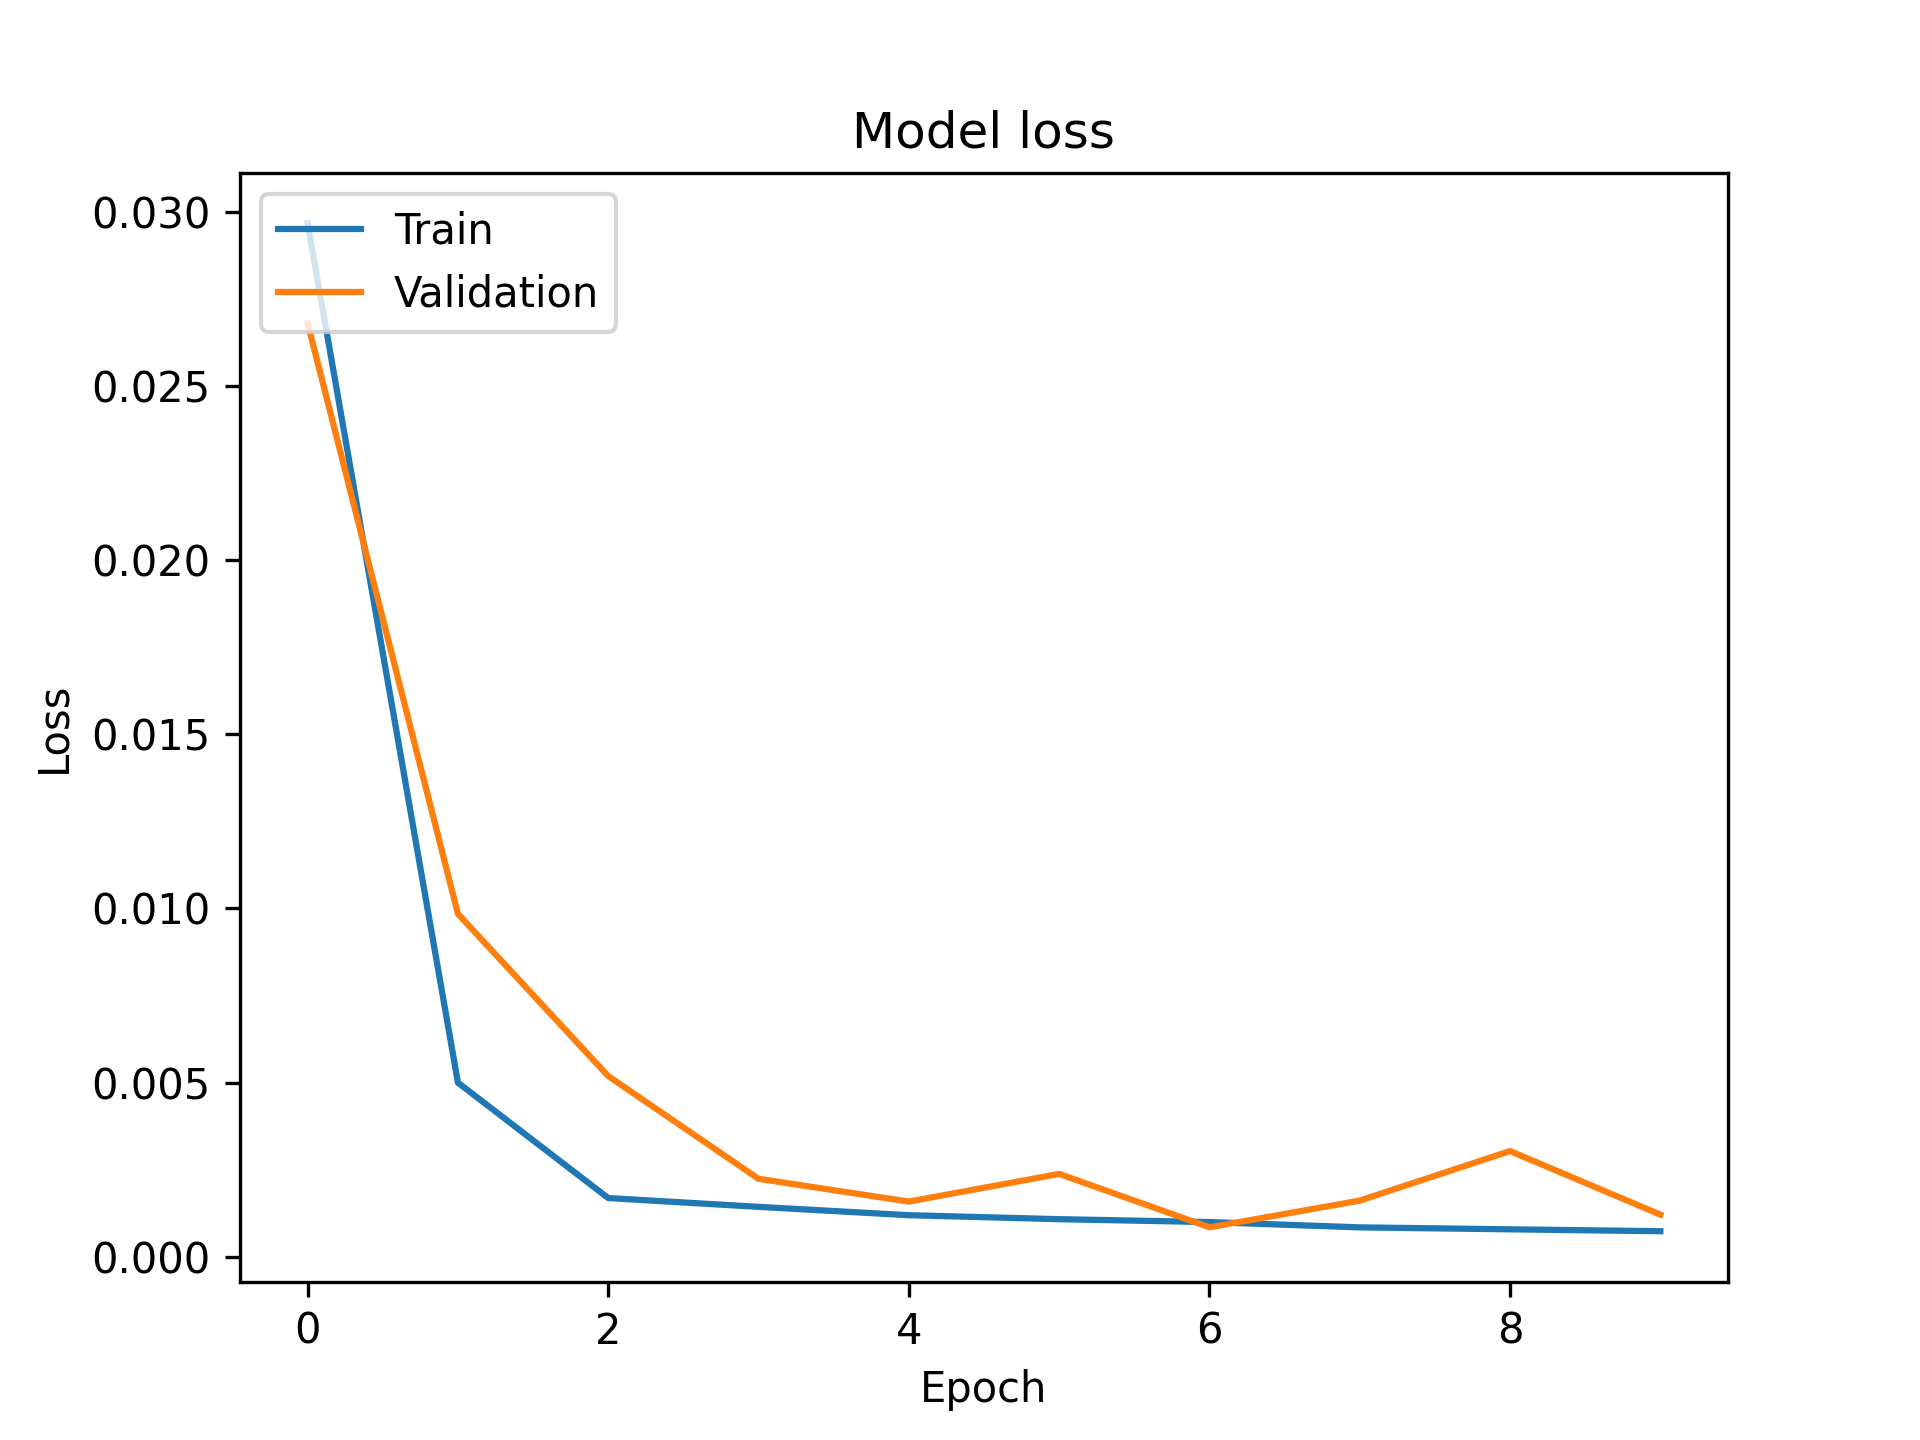
\includegraphics[width=0.8\linewidth]{images/SRResNet_losses.png}
  \caption{The training and validation losses for the SRResNet model for the x2 upscaling}
  \label{fig:SRResNet_losses}
\end{figure}
However, the fact that the model was trained using the mean square error as a loss metric results in the super-resolution to not be completely satisfactory. The model is not able to capture all the fine details contained in the original image. For example, the folds of the brain are not clearly delineated. This does not come as a complete surprise, given the simplicity of the mean squared error function and previous findings by Ledig et al.\cite{ledig2017photo}. However, the general outline of the morphological structures is well preserved. Some of the results can be seen in Fig. \ref{fig:SRResNet_ouput}

\begin{figure}[t]
    \centering
    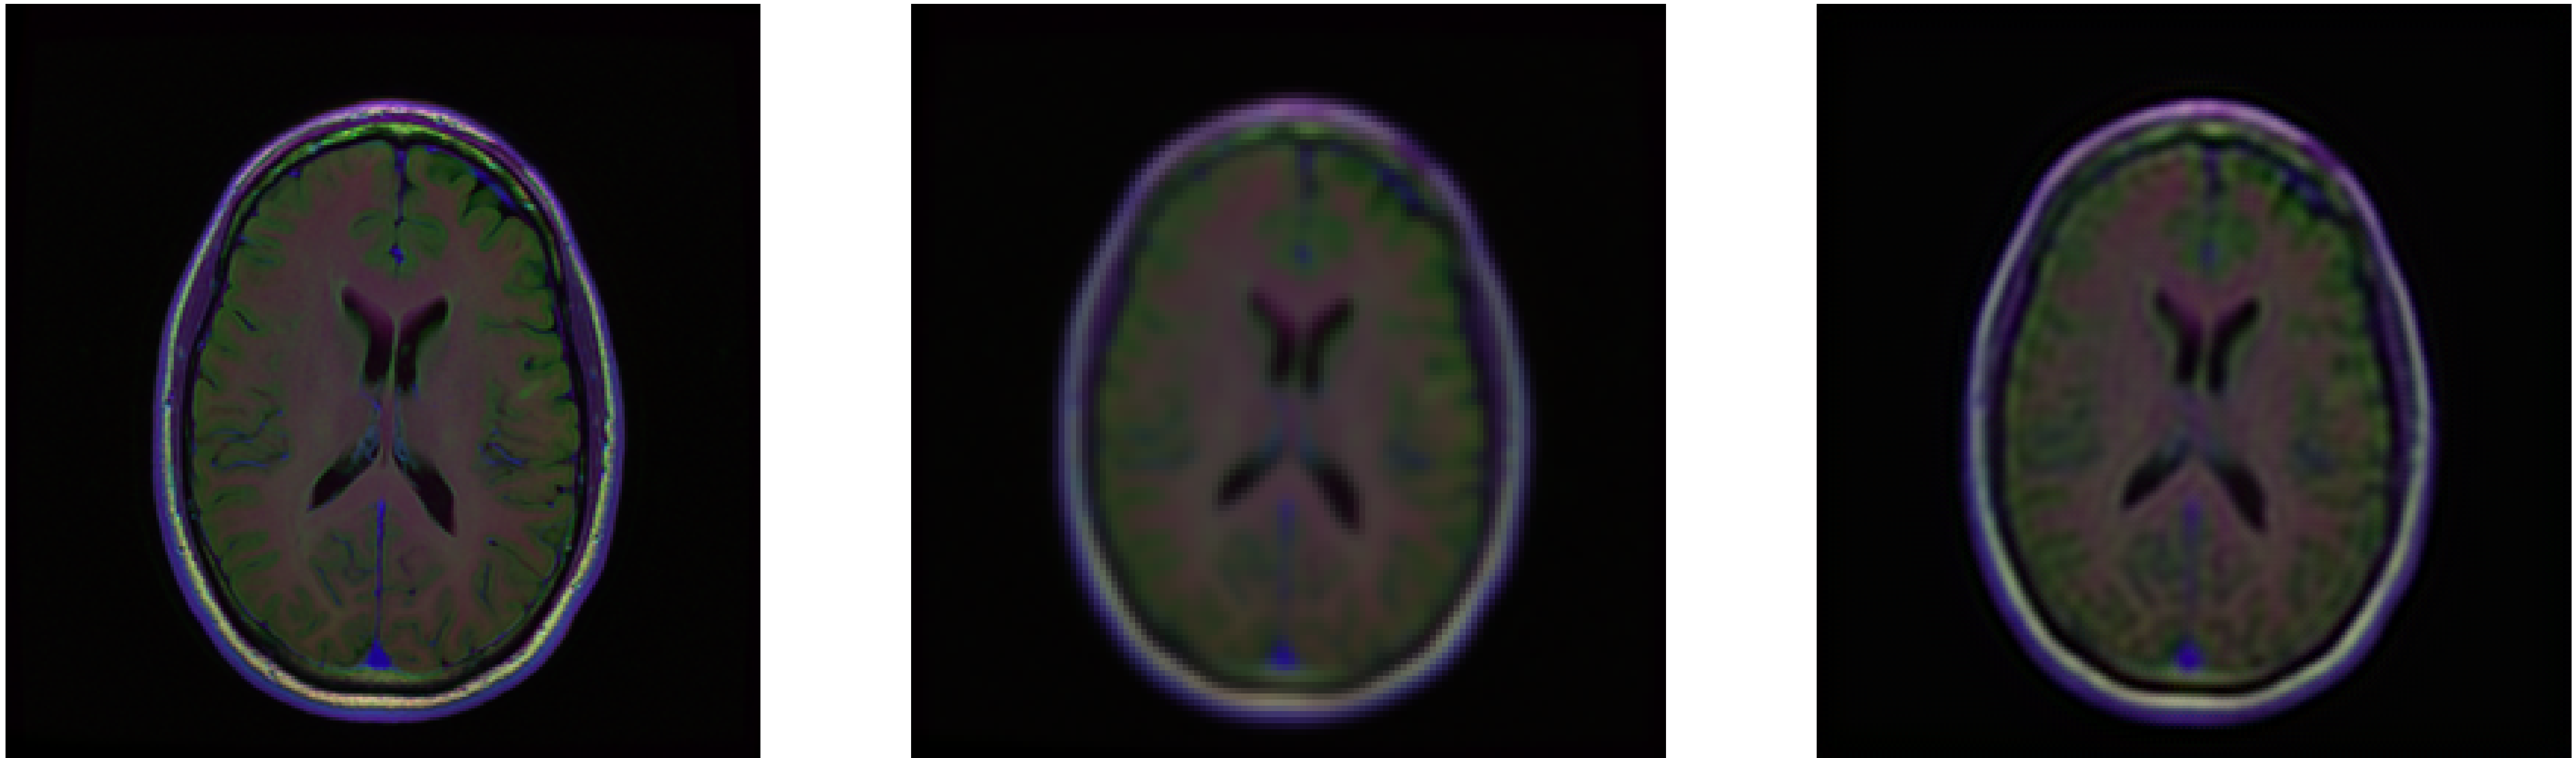
\includegraphics[width=0.85\linewidth]{images/SRResNet_epoch6_cropped.png}
    \caption{The results of the x2 upsampling of the SRResNet model from epoch 6: The original high resolution image (left), the low resolution input image (middle), and the final super resolution image (right)}
    \label{fig:SRResNet_ouput}
\end{figure}

\subsubsection{Upsampling x4}
The super-resolution model using the x4 upscaling was not as successful. The training process was successful, with both the the training and validation loss decreasing over the epochs, as can be seen in Fig. \ref{fig:SRResNet_64_losses}. In contrast to the the x2 upscaling model, there does not seem to be overfitting, which may imply that the model could be marginally further improved by training for a longer time.
\begin{figure}[t]
    \centering
    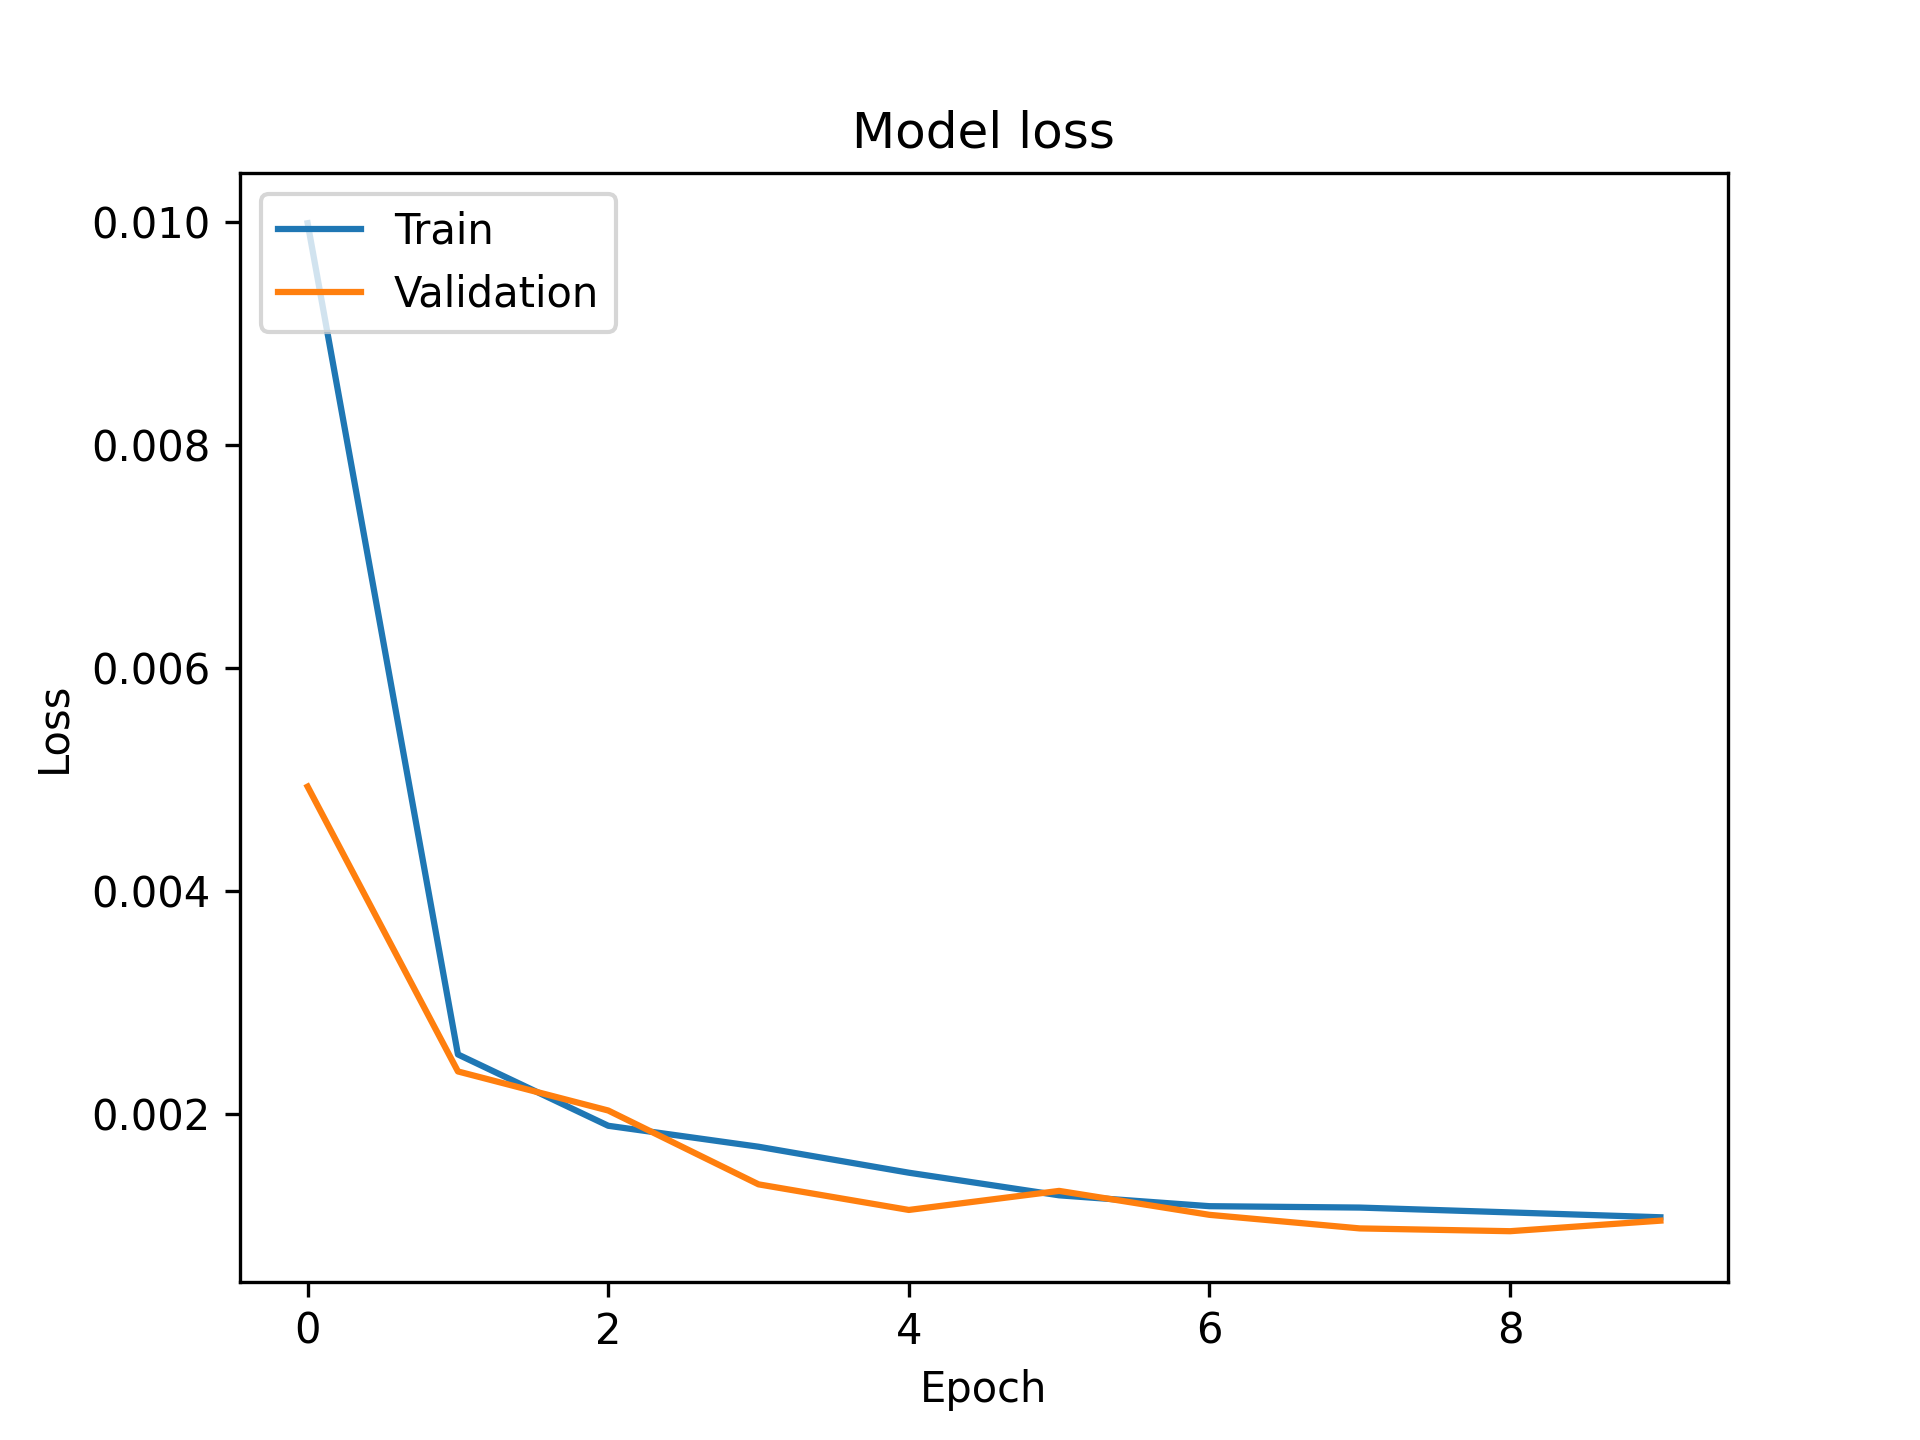
\includegraphics[width=0.8\linewidth]{images/SRResNet_64_losses.png}
    \caption{The training and validation losses for the SRResNet model for the x4 upscaling}
    \label{fig:SRResNet_64_losses}
\end{figure}

Here, the outputs displayed in Fig. \ref{fig:SRResNet_64_output} are much less satisfactory as with the x2 upsampling. It is no longer valid to state that the morphological features are well maintained in the output. 
\begin{figure}[t]
    \centering
    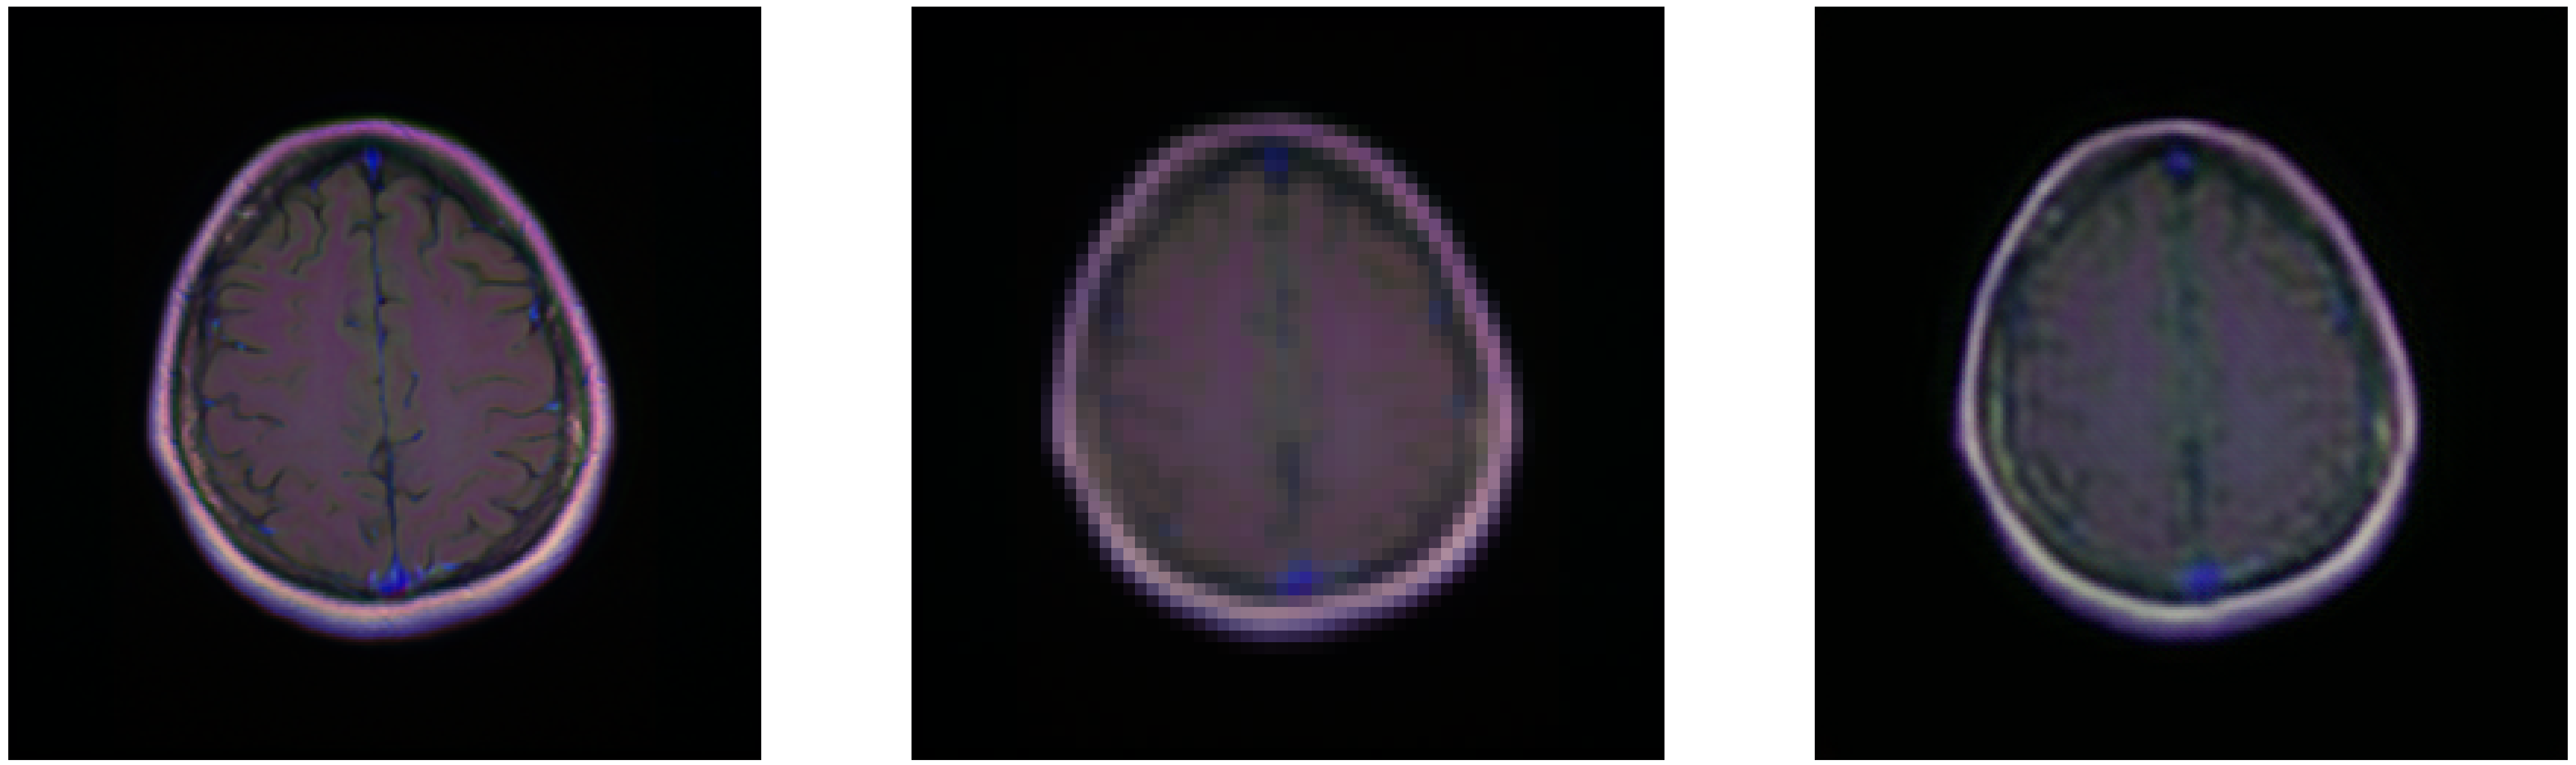
\includegraphics[width=0.85\linewidth]{images/SRResNet_64_epoch9_cropped.png}
    \caption{The results of the x4 upsampling of the SRResNet model from epoch 9: The original high resolution image (left), the low resolution input image (middle), and the final super resolution image (right)}
    \label{fig:SRResNet_64_output}
\end{figure}

\subsection{SRGAN}
The SRGAN model was trained to perform x2 upsampling. Many hyperparameters were attempted; the configuration that was ultimately retained is given in Table \ref{tab:hyperparams}. The training was not very satisfactory and it proved not feasible to train a model that is able to perform the super-resolution. In general, it is difficult to interpret the loss functions that are generated during the training of a GAN (\textit{vide infra}) and the performance should rather be assessed by means of visual inspection of the outputs. A decreasing generator loss, in particular, is not evidence of improving image quality: it indicates only that the generator is currently winning against a discriminator that may itself have degraded. With this caveat, we observe that both the generator loss and discriminator loss generally decrease throughout the training process, as illustrated in Fig. \ref{fig:SRGAN_losses}.
\begin{figure}[t]
    \centering
    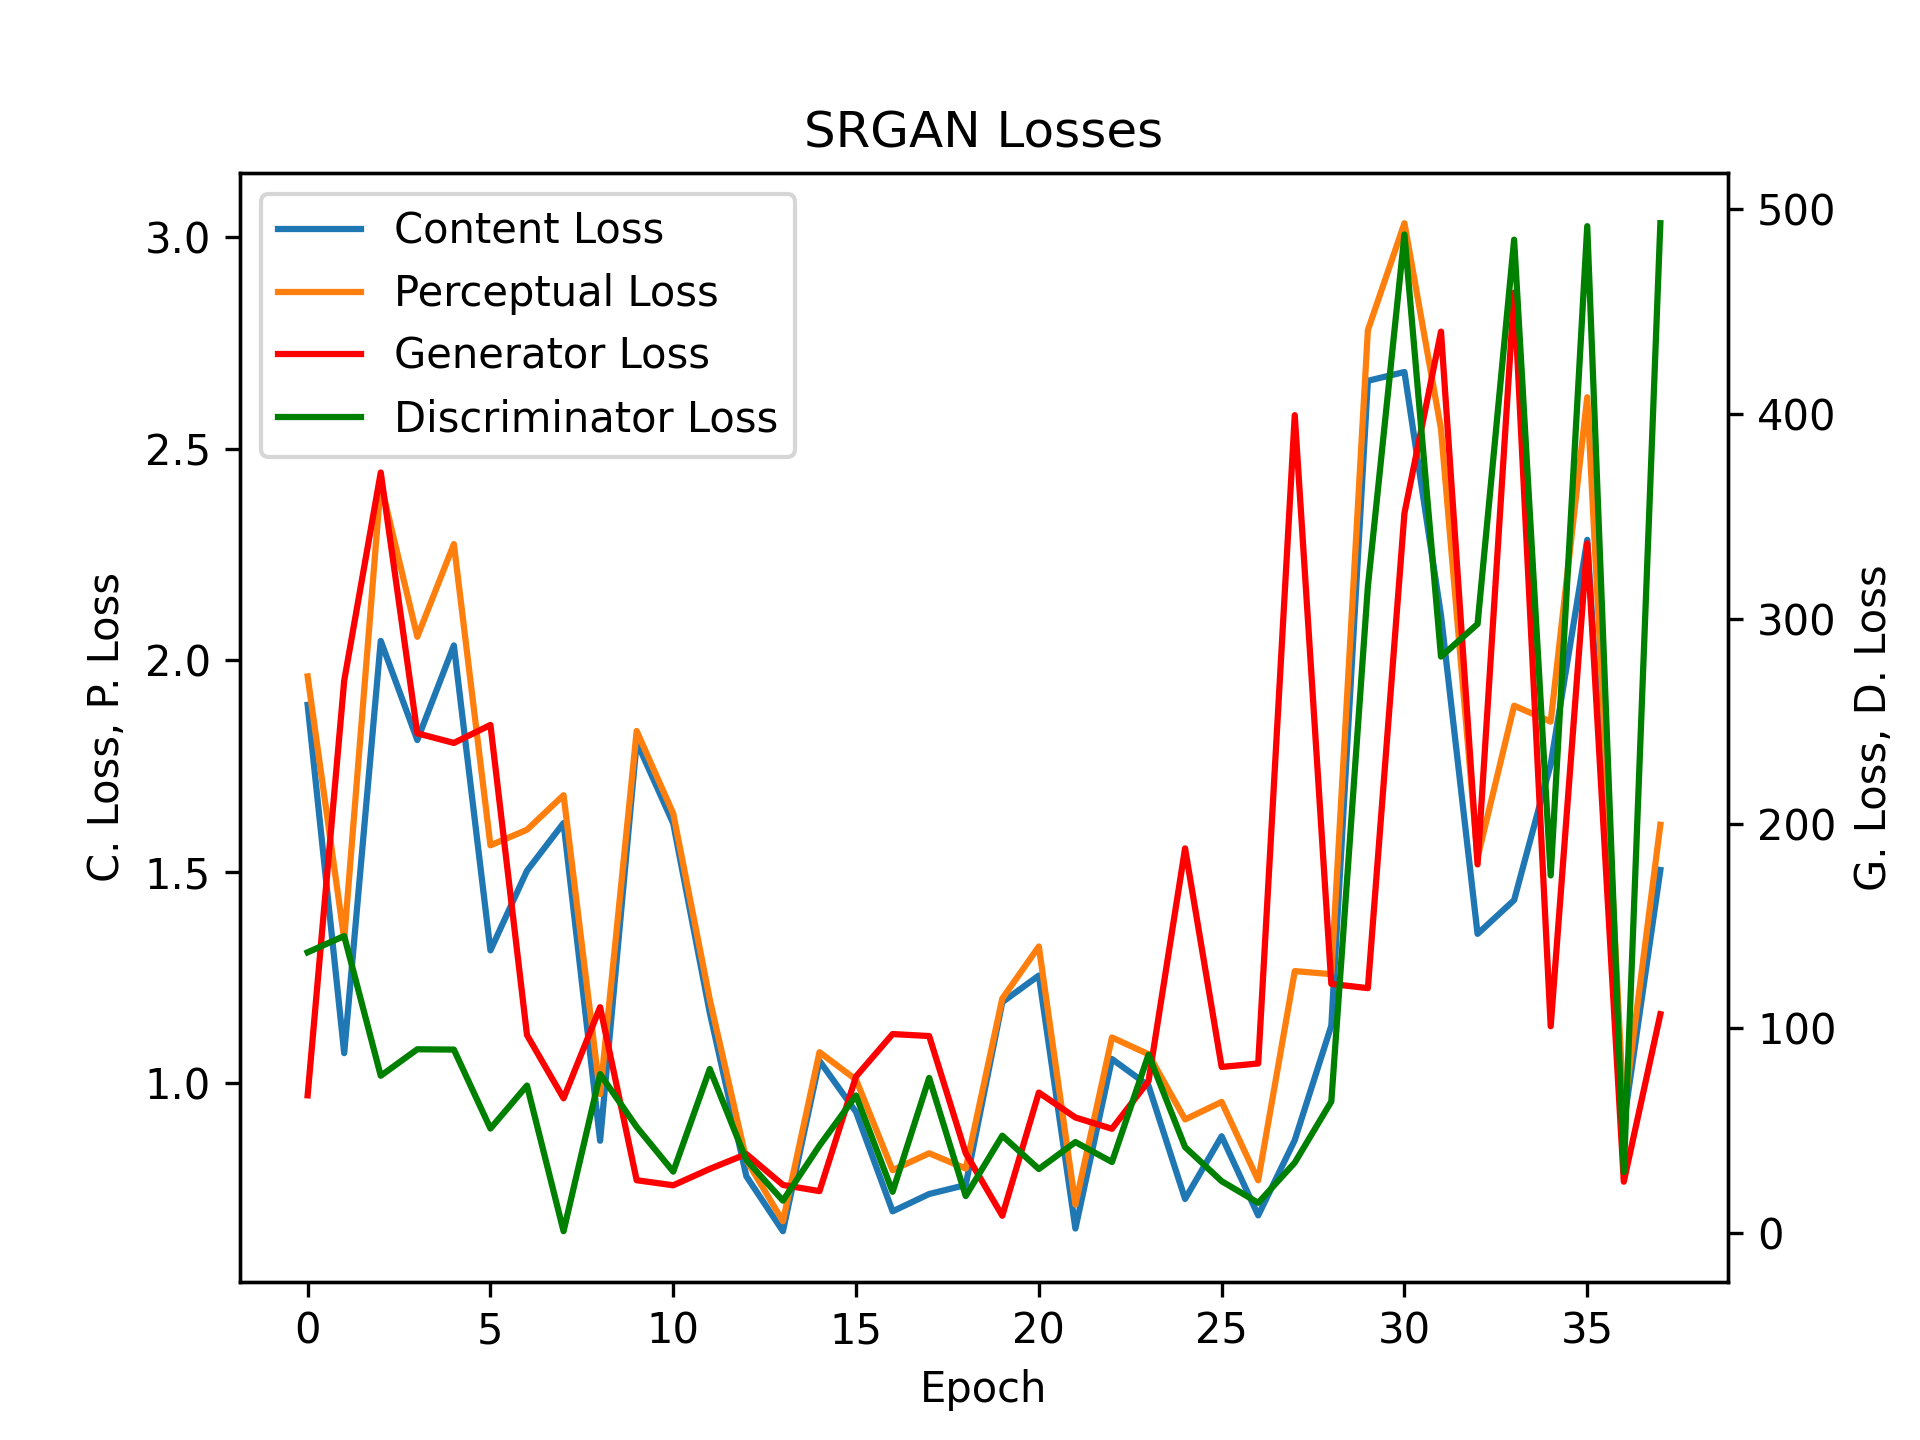
\includegraphics[width=0.8\linewidth]{images/SRGAN_losses.png}
    \caption{The generator and discriminator losses for the SRGAN model for the x2 upsampling}
    \label{fig:SRGAN_losses}
\end{figure}

However, the model does not converge during the training process, as can be observed from Fig. \ref{fig:SRGAN_outputs}. The model is clearly able to recognize some of the morphological features presented in the input images, but it is not able to train the generator to output an image that is similar to the original input image. It is possible to see how the GAN progresses from low-level features to more complex and specific features, where it learns to output some images resembling the original input. However, as the training continues, the model becomes unstable, which can be seen both in the visual outputs and the loss functions. In general, the training process is very variable from run to run and the instability is not easily reproducible. It could be possible that the MRI images are simply too different from the input data of the VGG19 model, which are normal pictures. In this case, the perceptive loss function would cause the entire model to become unstable during training.

\begin{figure*}[t]
    \centering
    \begin{subfigure}{0.32\textwidth}
        \centering
        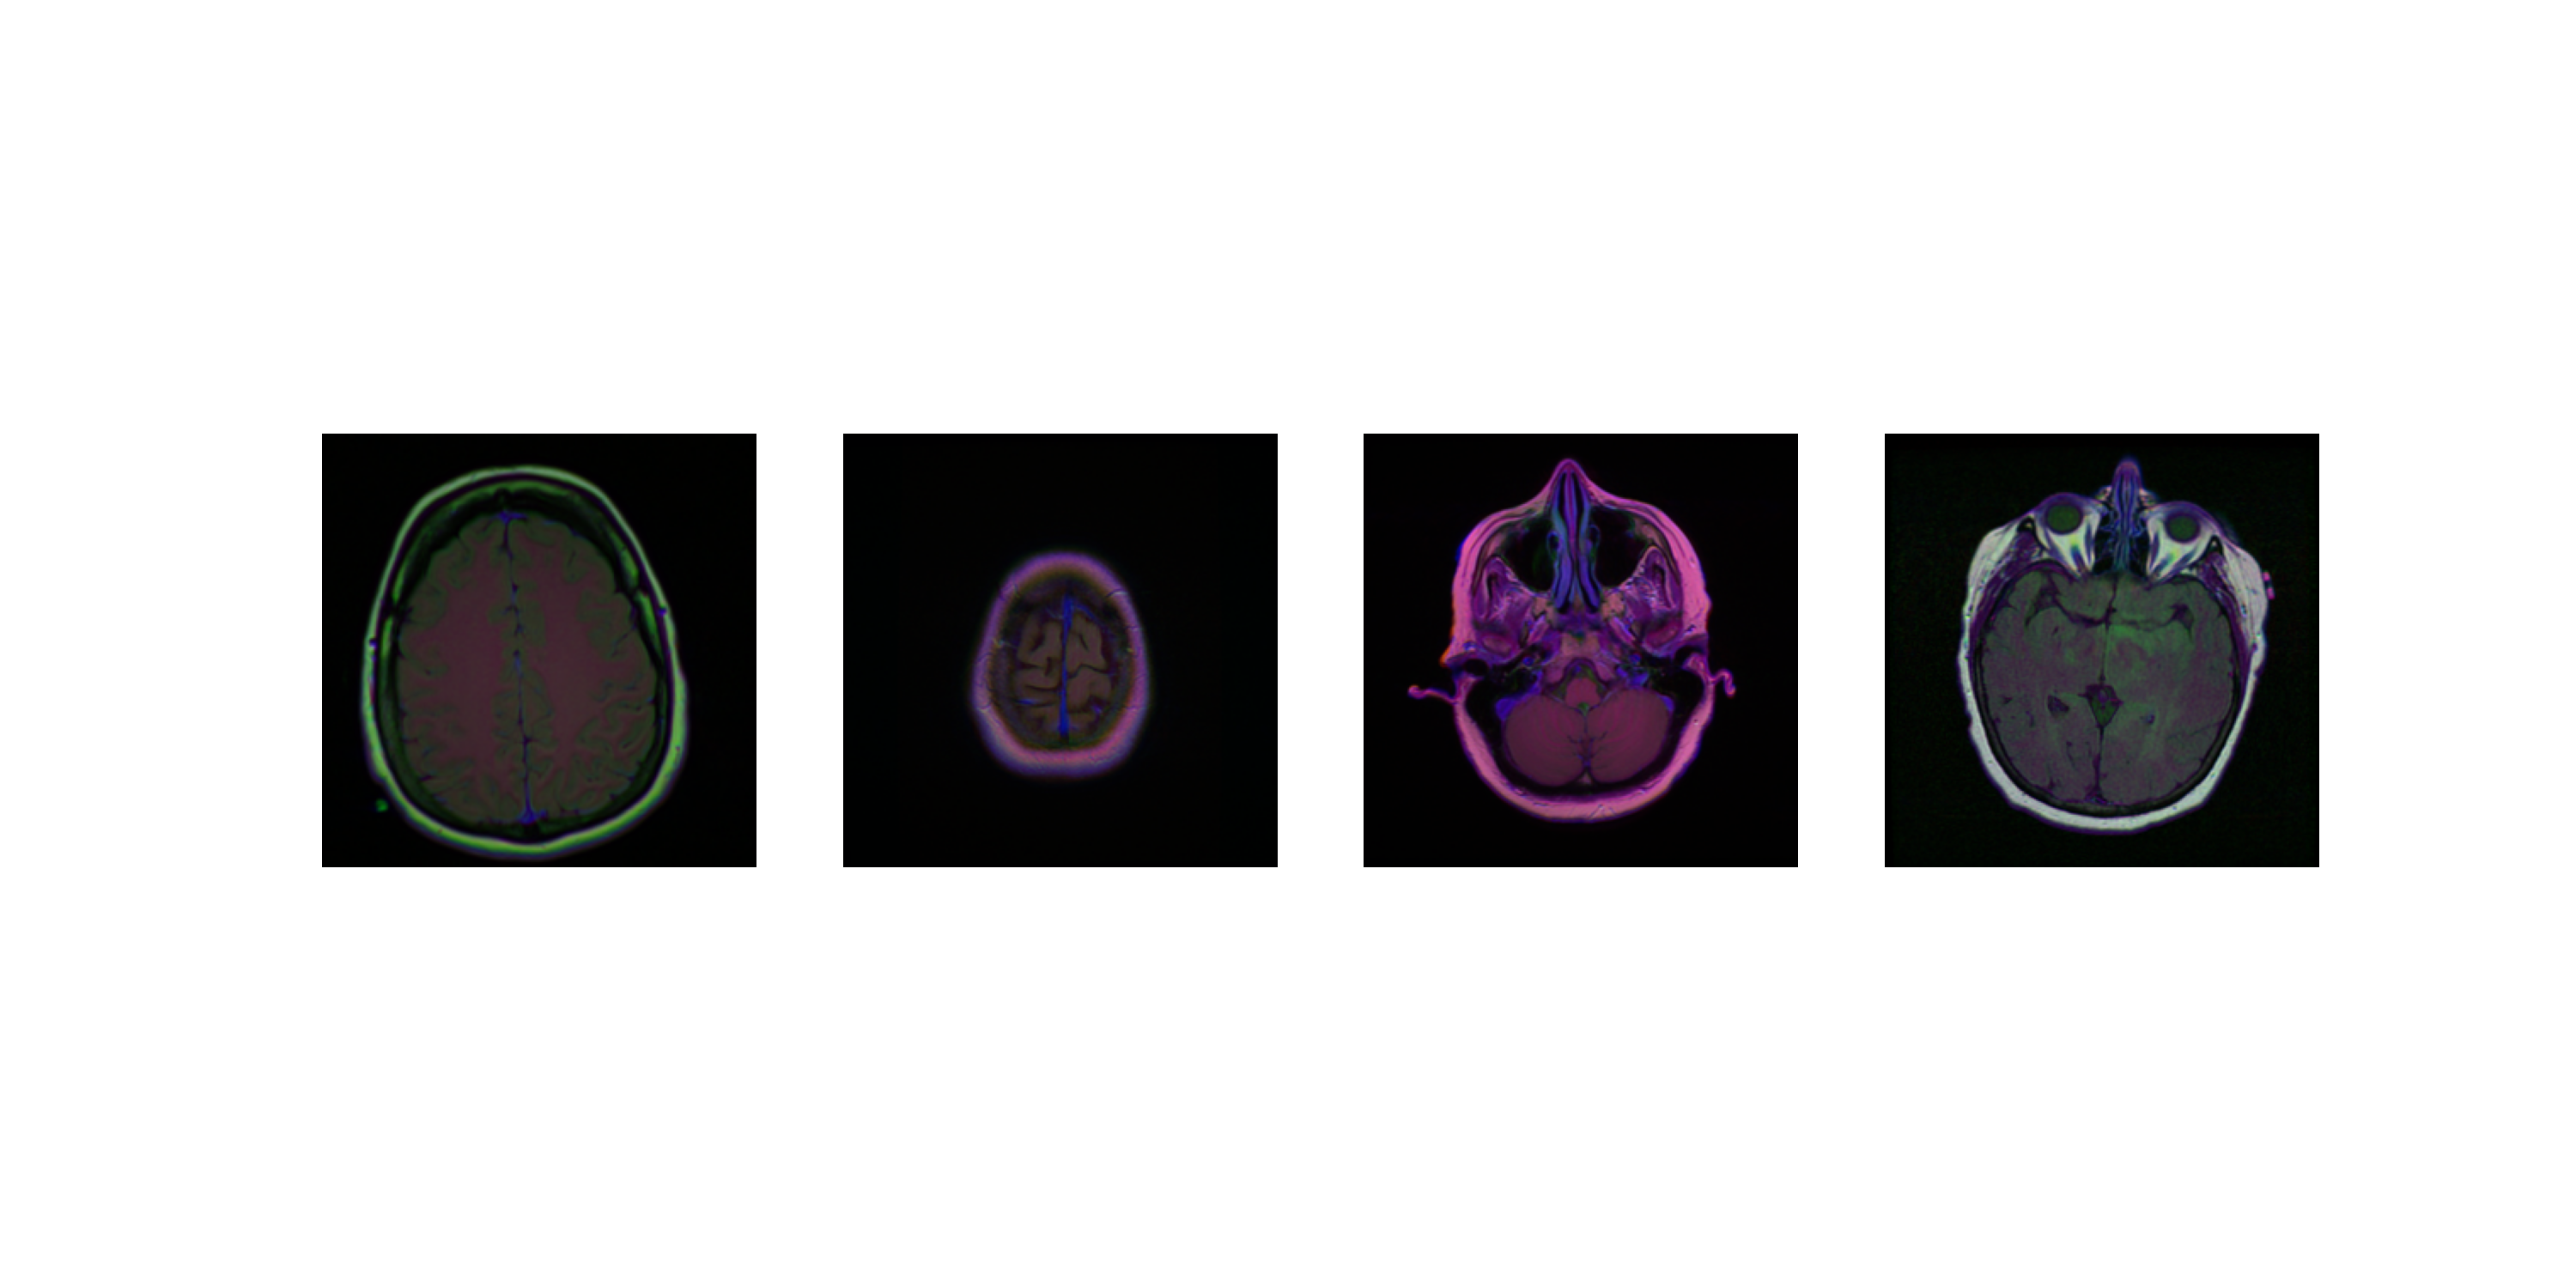
\includegraphics[width=\linewidth, trim=75 122 75 122, clip]{images/hr_1700.png}
        \caption{Ground-truth HR images}
    \end{subfigure}
    \hfill
    \begin{subfigure}{0.32\textwidth}
        \centering
        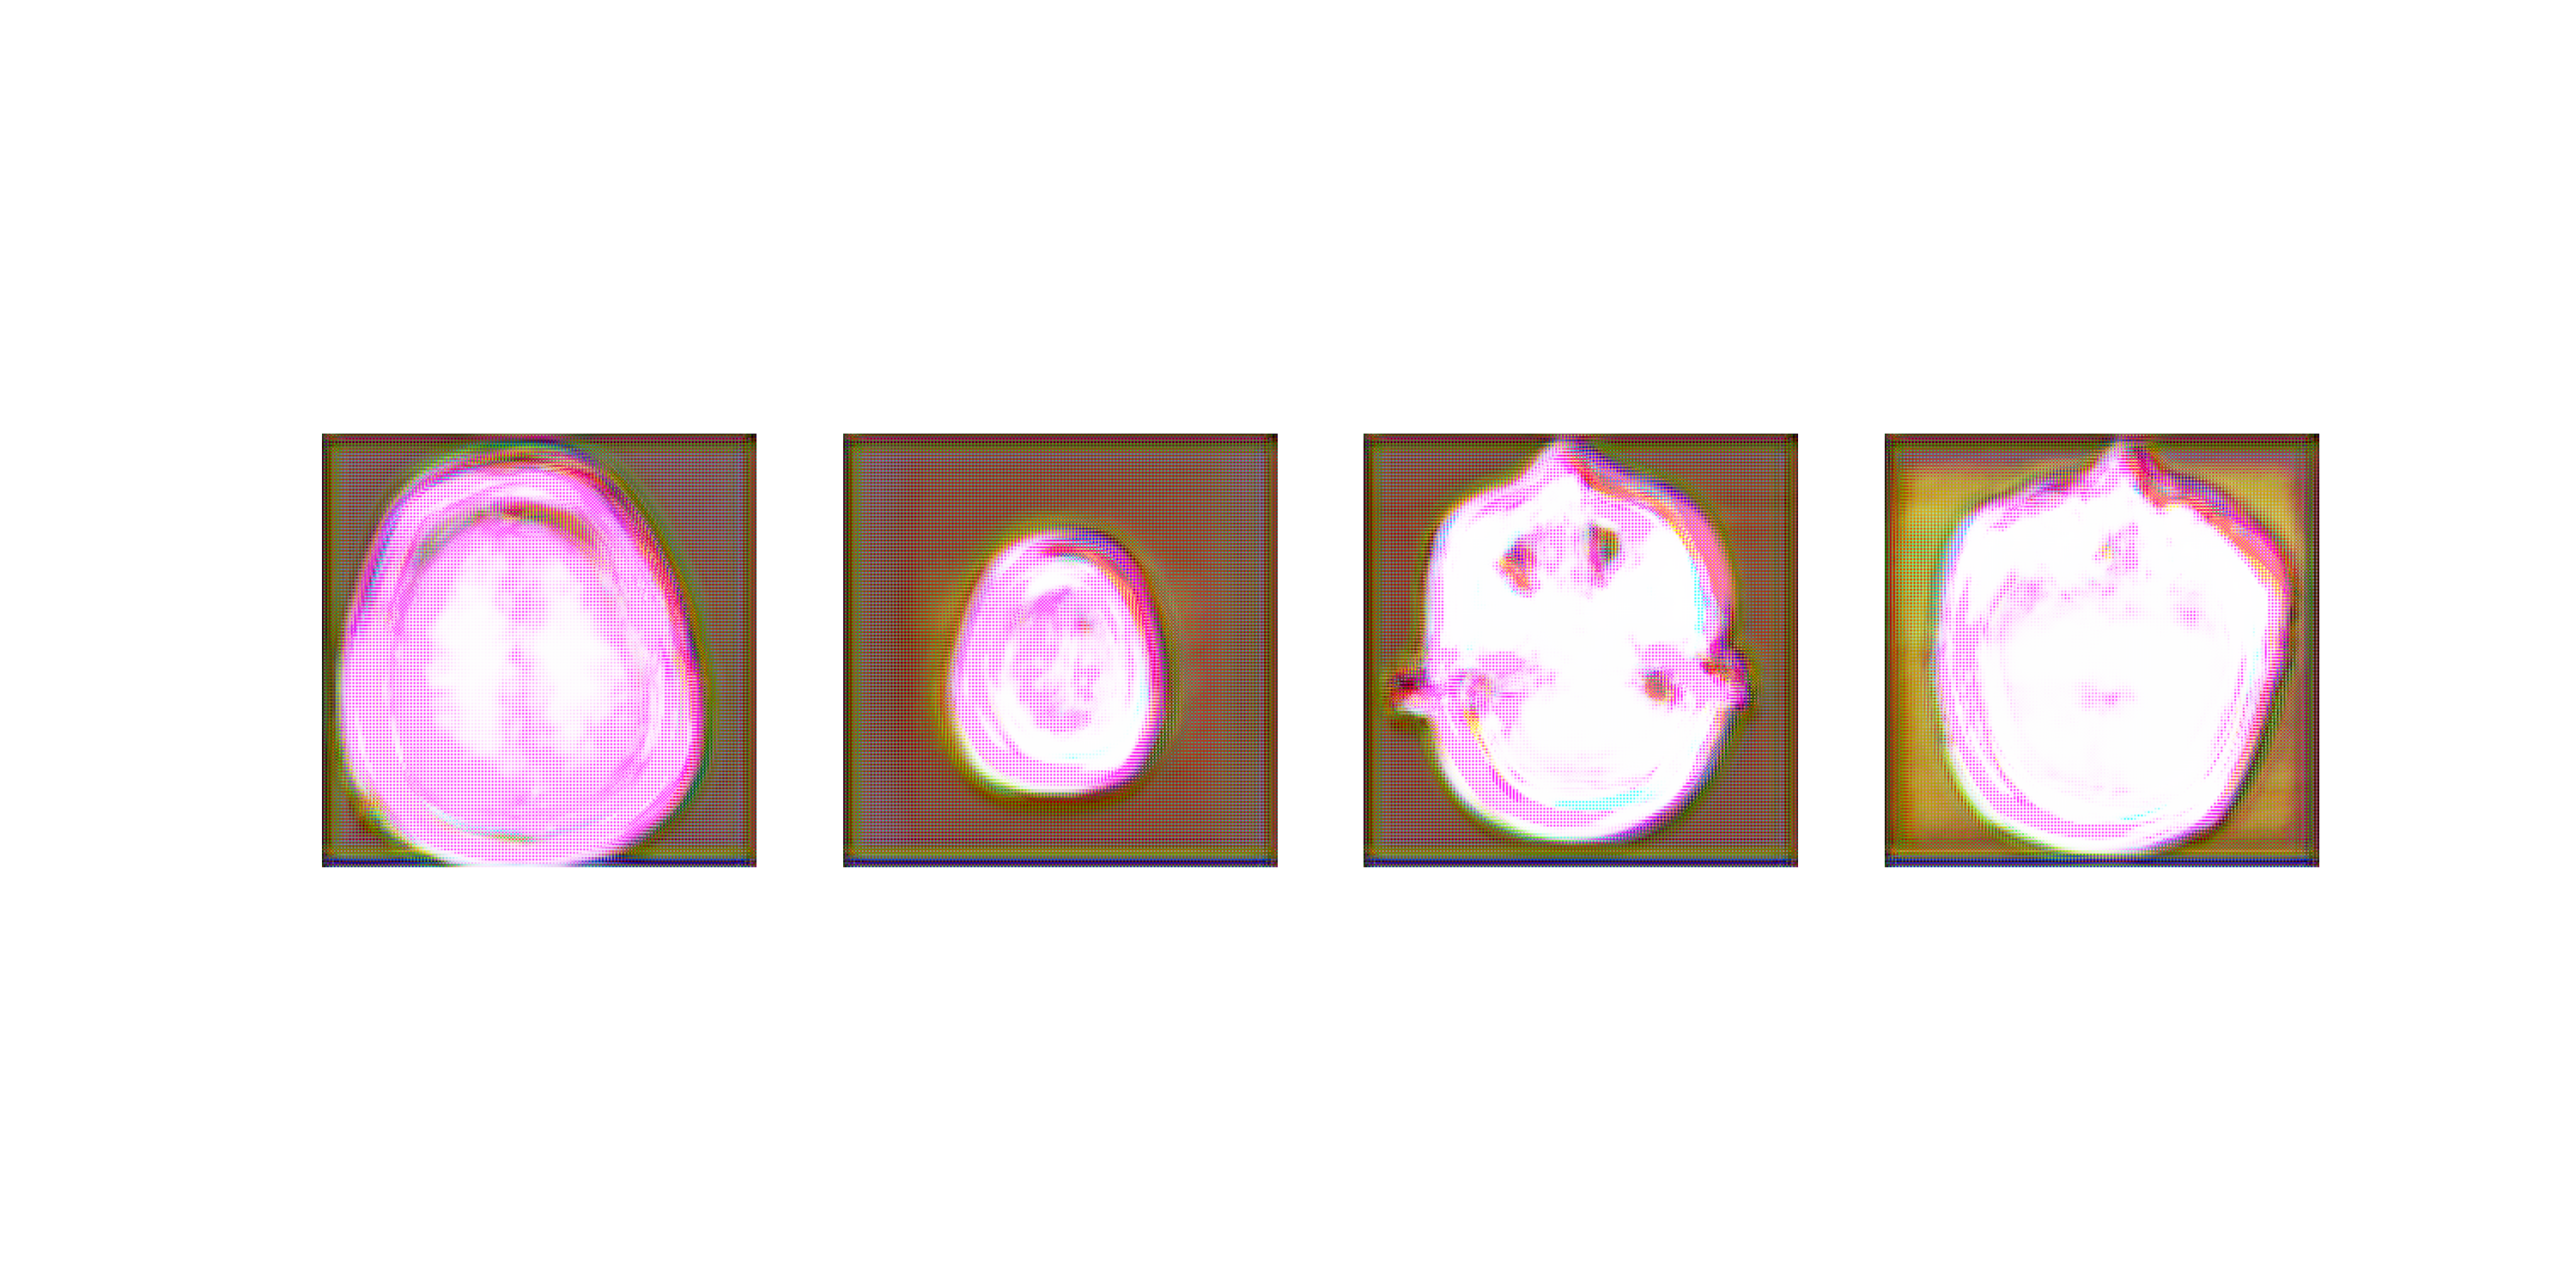
\includegraphics[width=\linewidth, trim=75 122 75 122, clip]{images/sr_100.png}
        \caption{Step 100}
    \end{subfigure}
    \hfill
    \begin{subfigure}{0.32\textwidth}
        \centering
        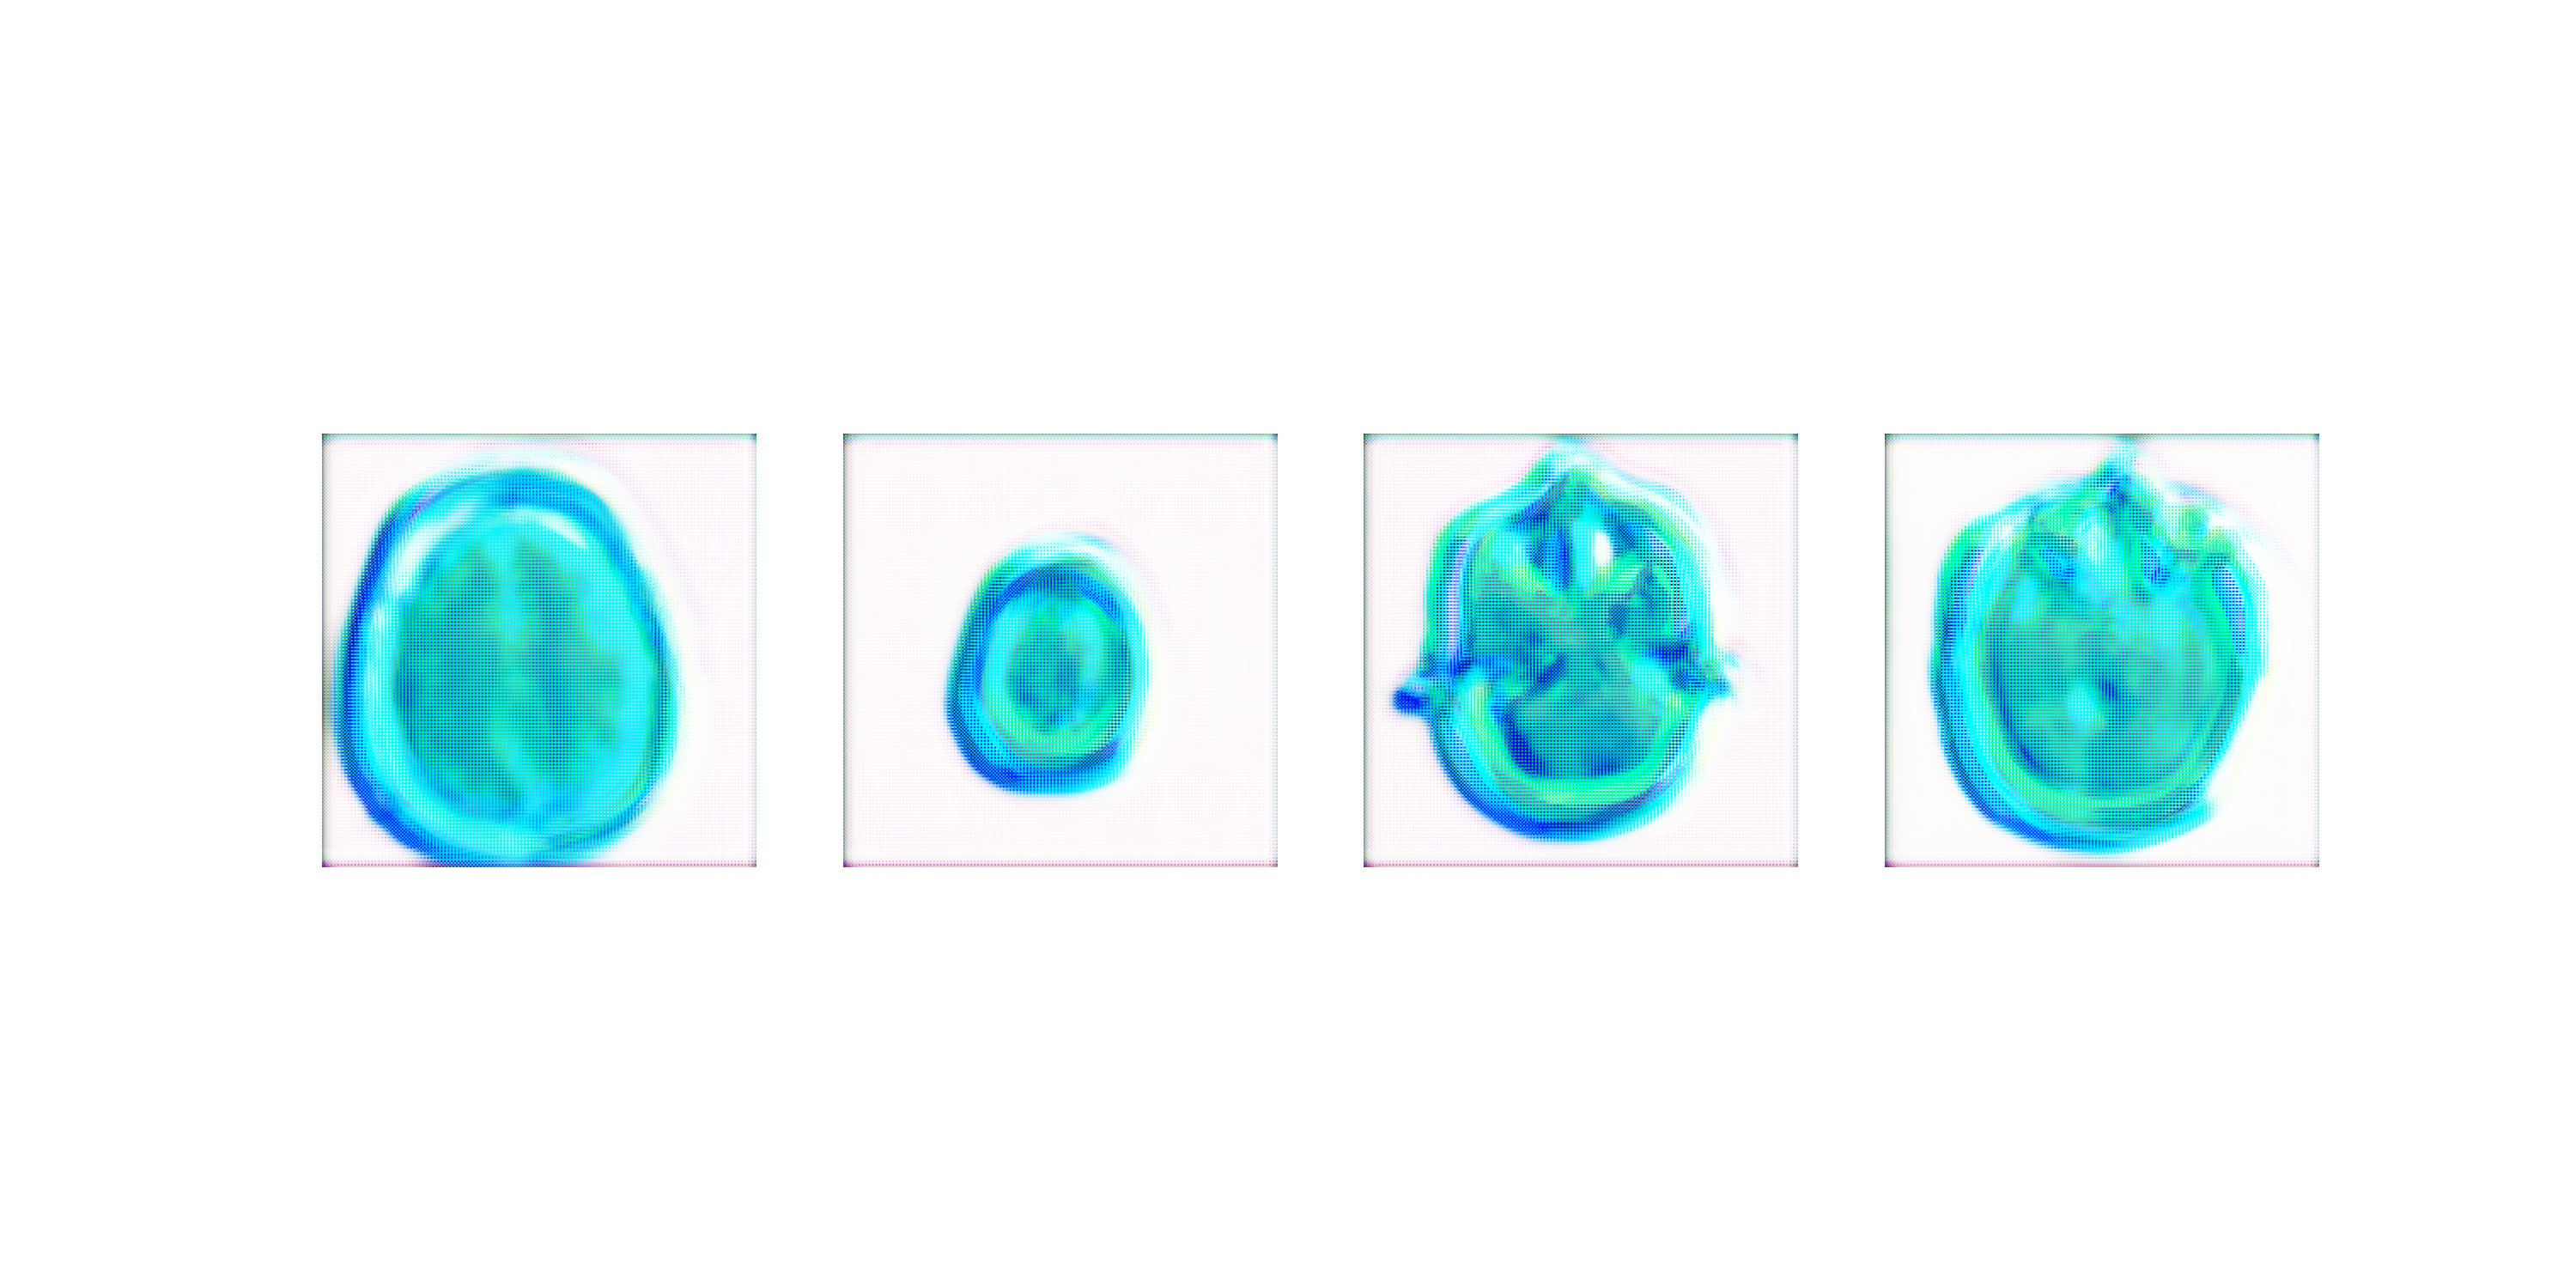
\includegraphics[width=\linewidth, trim=75 122 75 122, clip]{images/sr_200.png}
        \caption{Step 200}
    \end{subfigure}

    \vspace{0.6em}

    \begin{subfigure}{0.32\textwidth}
        \centering
        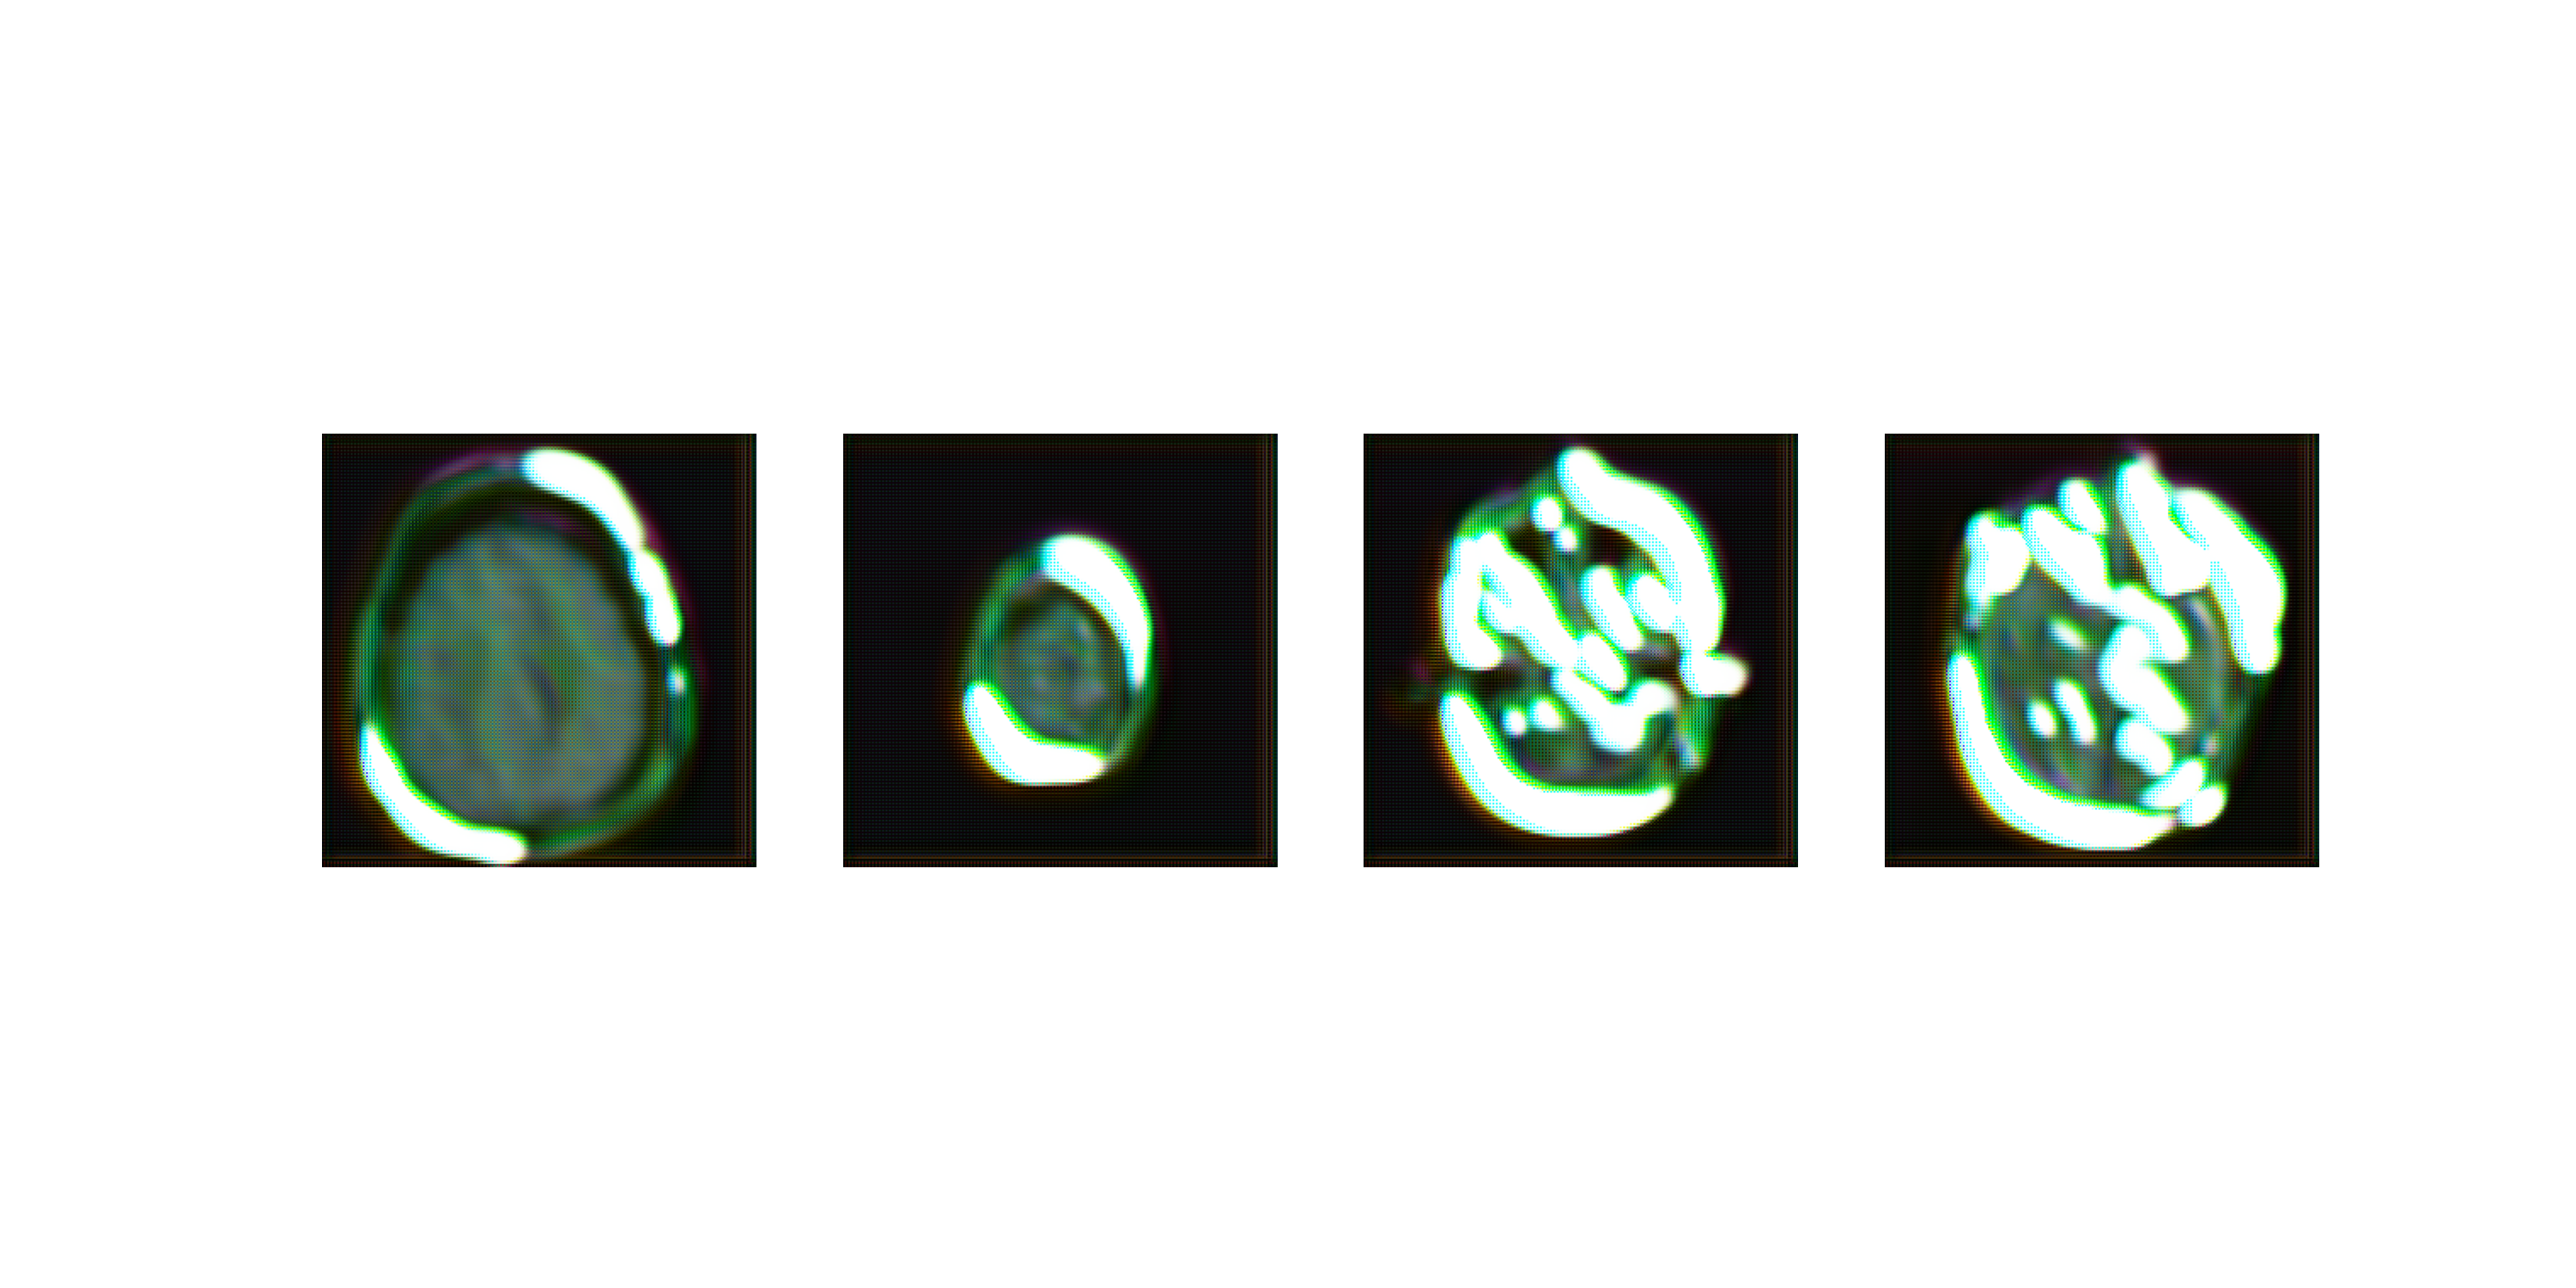
\includegraphics[width=\linewidth, trim=75 122 75 122, clip]{images/sr_700.png}
        \caption{Step 700}
    \end{subfigure}
    \hfill
    \begin{subfigure}{0.32\textwidth}
        \centering
        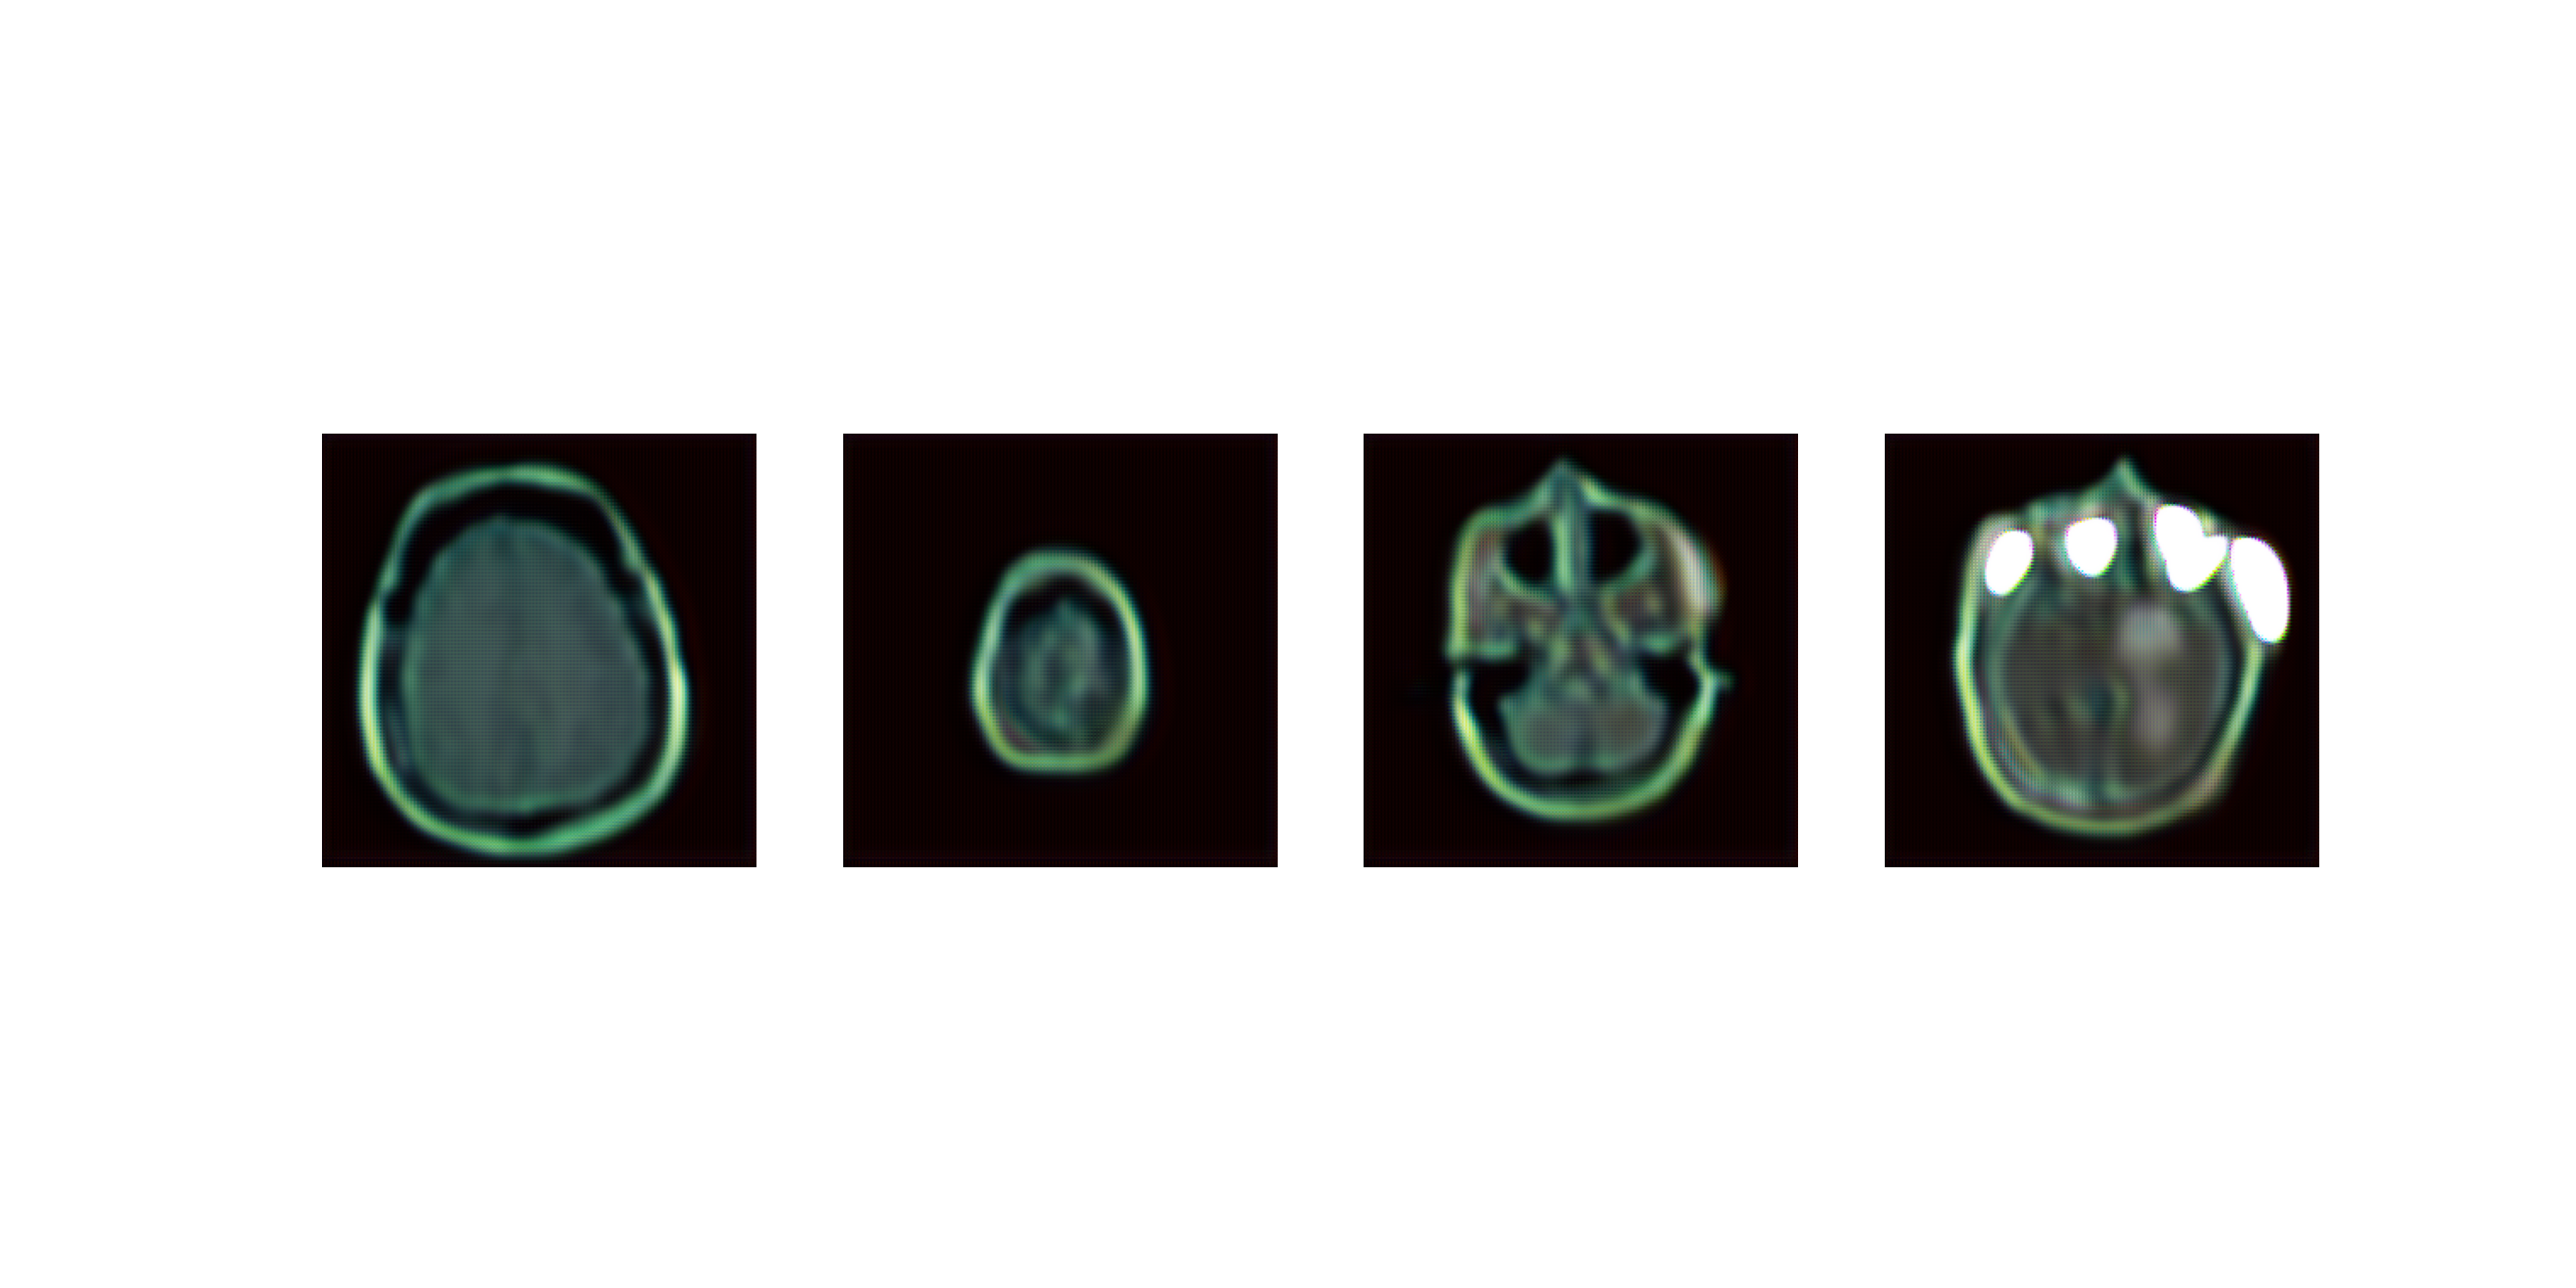
\includegraphics[width=\linewidth, trim=75 122 75 122, clip]{images/sr_1200.png}
        \caption{Step 1200}
    \end{subfigure}
    \hfill
    \begin{subfigure}{0.32\textwidth}
        \centering
        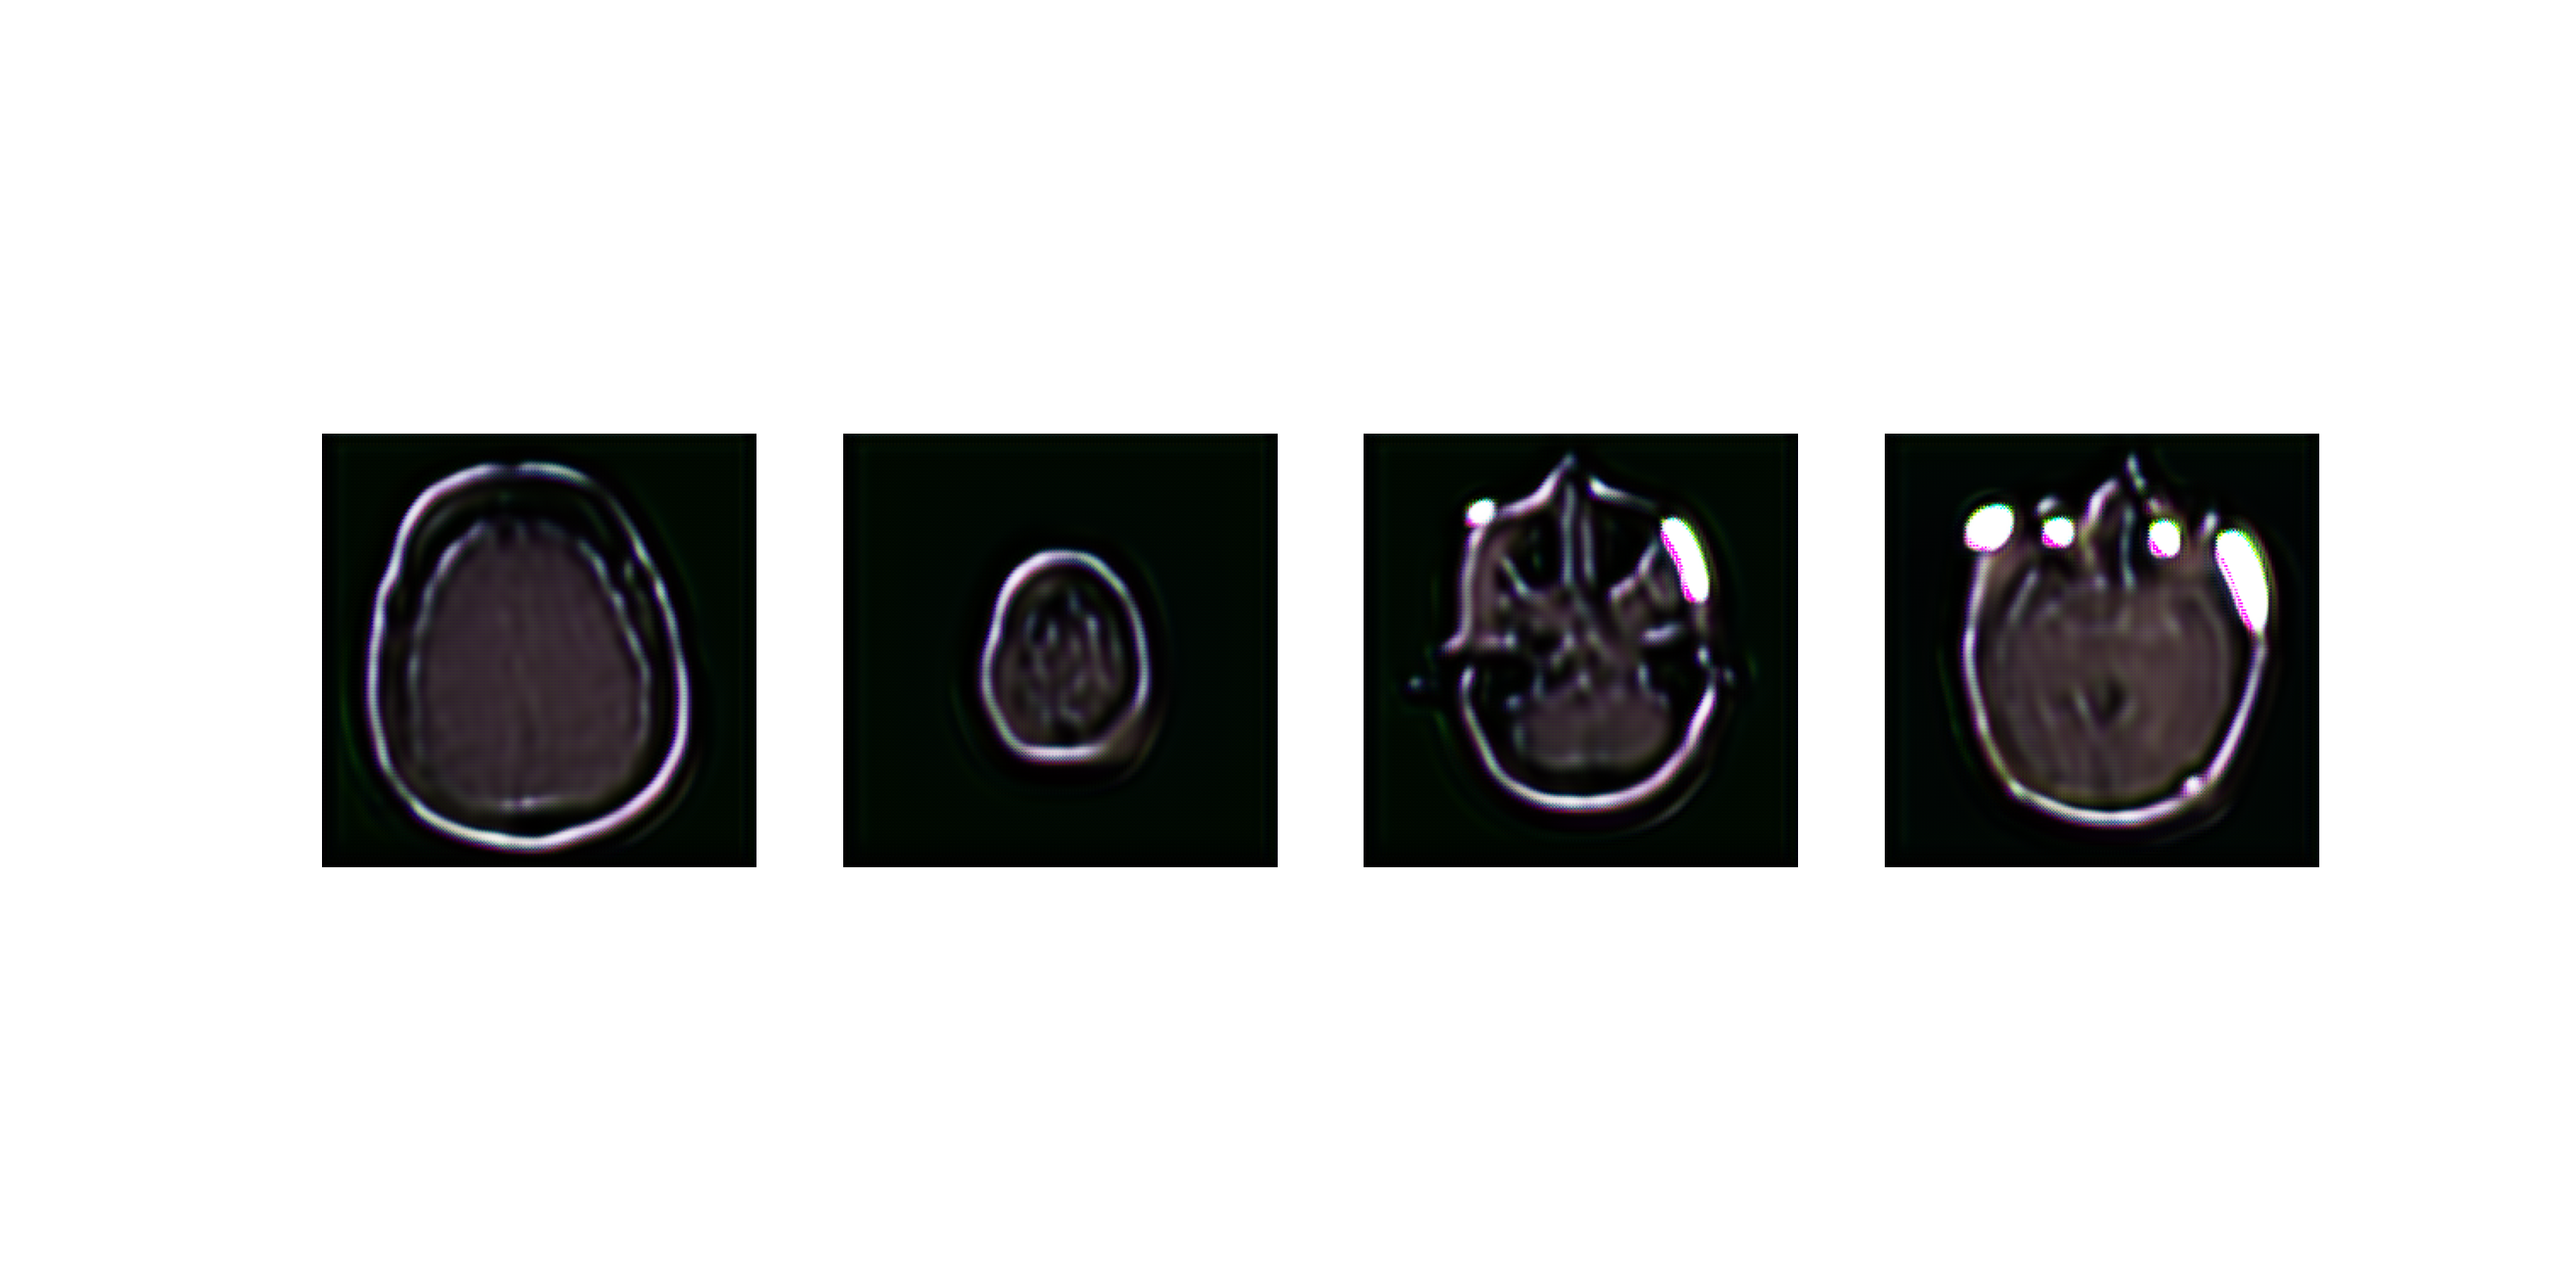
\includegraphics[width=\linewidth, trim=75 122 75 122, clip]{images/sr_3000.png}
        \caption{Step 3000}
    \end{subfigure}
    \caption{Ground-truth high resolution images (a) and SRGAN generator outputs at increasing training steps (b)--(f). The model recovers coarse morphological structure early, but destabilizes as training proceeds.}
    \label{fig:SRGAN_outputs}
\end{figure*}


\section{Limitations}
\label{sec:limitations}

\subsection{Difficulty of Training GANs}
While GANs have been seen to generate very realistic results, they are notoriously hard to train. As stated in a follow-up paper by Salimans et al. \cite{salimans2016improved}, GANs are designed to find a Nash equilibrium of a non-convex game with continuous high-dimensional parameters. Meanwhile gradient descent - the method by which GANs are typically trained - is designed to minimize the provided loss function, not to find a Nash equilibrium of a game. This causes issues with convergence, as when the loss of one network goes down, the other will go up correspondingly. This unfortunate consequence of GAN architecture causes them to be very unstable in training and extremely sensitive to hyper parameters and initial conditions. 
\subsection{Initial Architecture}
Some difficulties were encountered during the initial training process. The first GAN architecture we attempted to train was a much simpler one than outlined in this paper, with both the generator and discriminator containing four 2D convolutional layers that mirror each other in architecture but perform their respective mappings. Outputs from this were promising for the first few epochs, but quickly descended into instability. 
\begin{figure}[t]
    \centering
    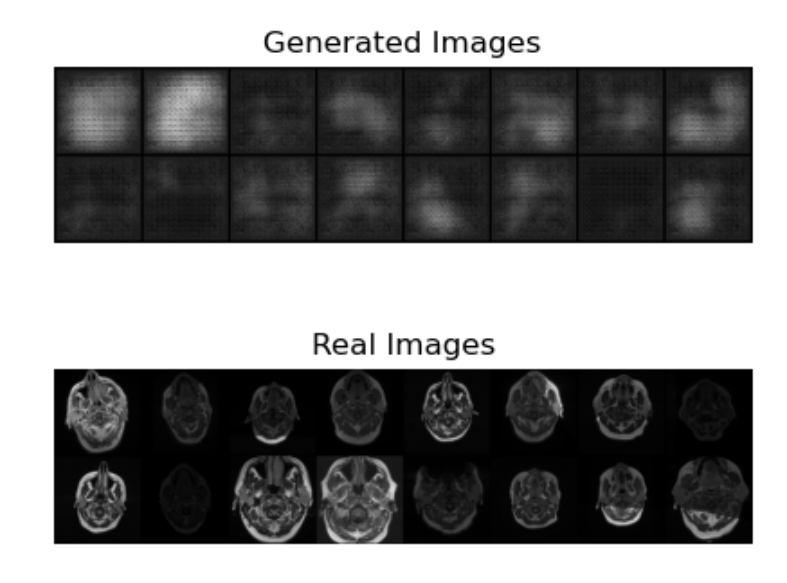
\includegraphics[width=0.9\linewidth]{images/limitation_1.png}
    \caption{Outputs from the original GAN}
    \label{fig:limitation-original-gan}
\end{figure}

We proceeded to follow the recommendations of Salimans et al. \cite{salimans2016improved} and add batch-normalization layers. However, with this architecture, we experienced some mode collapse difficulties. Mode collapse refers to the behavior where the generator finds some features that can fool the discriminator and repeatedly generates small variations of those without exploring the entire distribution of the data or diversifying the generated samples. This causes each of the generated images to be more or less identical.

\begin{figure}[t]
    \centering
    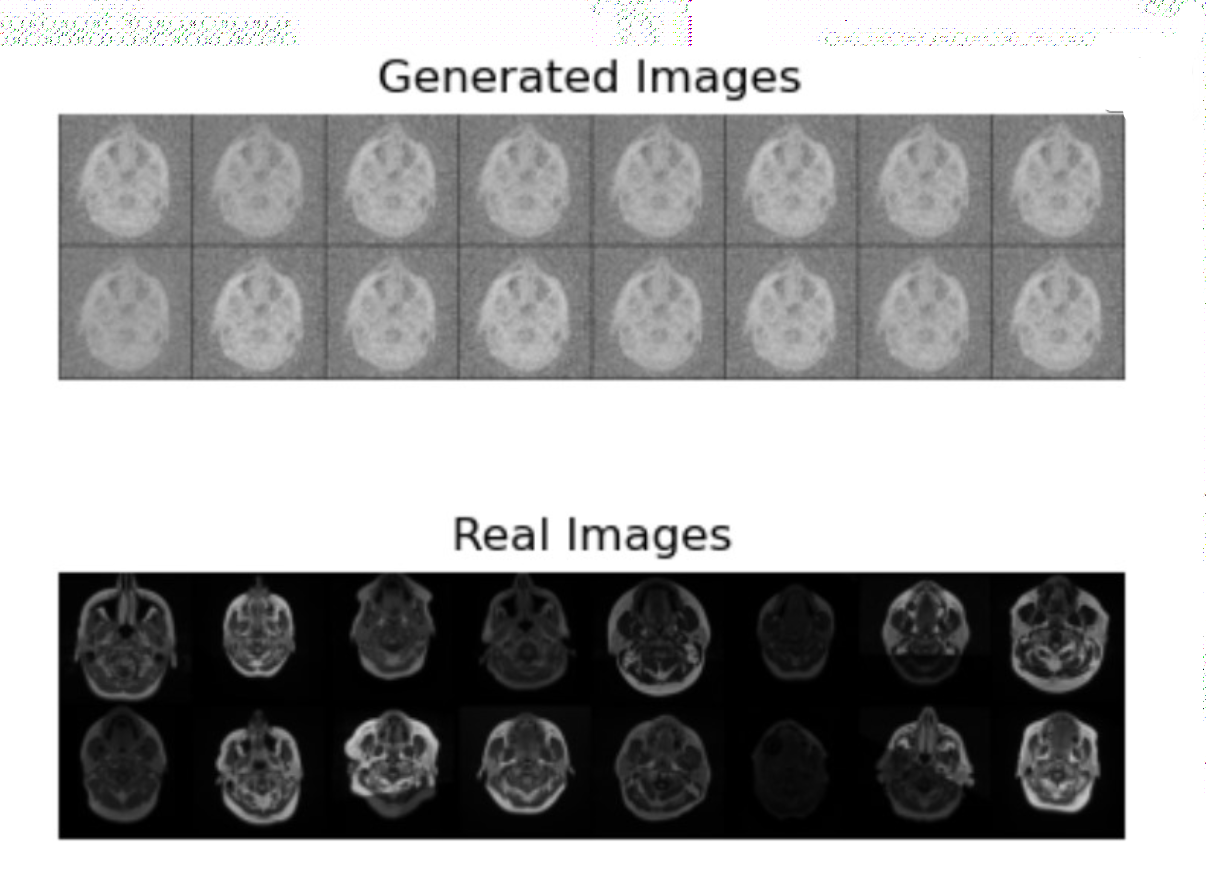
\includegraphics[width=0.9\linewidth, trim=0 0 0 23, clip]{images/limitation_2.png}
    \caption{Mode collapse illustrated by our primal GAN}
    \label{fig:limitation-mode-collapse}
\end{figure}

These results showed that it was necessary to explore more complex and deeper architectures, such as the one we have presented in this paper.

\subsection{Evaluation and Experimental Design}
Several limitations of this study are methodological rather than architectural, and they bound how strongly its conclusions can be stated.

First, no quantitative metric is reported. All comparisons in Section \ref{sec:results} rest on visual inspection of a small number of validation slices, which cannot distinguish a genuine improvement from a favourable choice of example, and which gives no basis for comparing the $\times 2$ and $\times 4$ models against each other or against a bicubic baseline. Computing PSNR and SSIM as defined in Eqs. \eqref{eq:psnr} and \eqref{eq:ssim} is the single most valuable addition that could be made to this work.

Second, the experiments use a train/validation split with no held-out test set, and model selection decisions, such as the identification of overfitting from epoch 6 onward, were made against the same validation split that is used to report results. The reported behaviour is therefore optimistic.

Third, the split is drawn at the level of individual slices rather than patients. Because adjacent slices from a single MRI session are highly correlated, near-duplicate images may appear in both the training and validation partitions, and the validation loss consequently overstates generalization to unseen patients. A patient-level split would be a more honest protocol, and we expect it to widen the gap between training and validation curves.

Fourth, the low-resolution inputs are synthesized by a fixed, known degradation. The network is asked only to invert a blur-and-decimate operator it has seen throughout training, so the results do not speak to performance on natively low-resolution acquisitions, where the degradation arises from $k$-space undersampling and motion.

Finally, the two configurations differ along several axes simultaneously, including loss function, learning rate, batch size, and validation fraction. This means the comparison between SRResNet and SRGAN is not controlled, and the failure of the adversarial model cannot be attributed to the perceptual loss alone.

\subsection{Domain Mismatch of the Perceptual Loss}
The content loss of Eq. \eqref{eq:content} is computed in the feature space of a VGG19 network trained to classify natural images from ImageNet. Its filters are tuned to the statistics of that domain: object contours, textures, and colour distributions that have little in common with greyscale-like MRI slices in which the same anatomical structure recurs in every image. Two consequences follow. The features extracted from an MRI slice may occupy a poorly conditioned region of the feature space, so that the gradient of $l_C$ carries little information about anatomical fidelity; and the fixed rescaling of activations by a constant factor, used to bring $l_C$ onto the same numerical scale as the adversarial term, is calibrated for natural-image activations and may not hold for this input distribution. If the two terms in Eq. \eqref{eq:perceptual} drift apart in magnitude during training, the effective adversarial weighting is no longer $10^{-3}$, which would be consistent with the instability observed in Fig. \ref{fig:SRGAN_outputs}.

\section{Conclusion}
The architecture of the generator (SRResNet) seems to be fundamentally solid for performing super-resolution of MRI brain images, which is supported by the results presented in section \ref{SRResNet}. This gives indication that the architecture can be used as a stepping stone for further research, though we stress that this assessment rests on visual inspection alone and remains to be confirmed quantitatively. At this point in time, the main limiting factor seems to be the loss function on which the generator is trained. The mean squared error gives reliable results, but suffers a more blurred output, which has previously been experienced in other research too and which follows from the fact that the pixel-wise optimum is the average of all plausible reconstructions. The VGG19-based GAN approach suffers from instability, and it proved more difficult to train the model than initially expected. Some conjectured causes for this instability include the inherent difficulties of training a GAN and the incompatibility of the VGG19 feature space with the MRI input images.

Immediate future work should begin with quantitative evaluation. Reporting PSNR and SSIM over a patient-level held-out test split, against a bicubic-interpolation baseline, would convert the qualitative claims made here into measurable ones and establish whether the SRResNet output improves on classical interpolation at all. Beyond this, more robust hyper-parameter tuning could address the instability, which in this work has been largely trial-and-error, and a controlled comparison that varies only the loss function would isolate the contribution of the adversarial objective. An attempt could also be made to use a more robust perceptive loss function. One possible strategy could be to fine-tune the VGG19 model on the original input set, or to replace it with a feature extractor trained on medical imagery, which would address the domain mismatch discussed in Section \ref{sec:limitations}. With an even more ambitious scope, some more advanced deep-learning techniques can be attempted to perform super-resolution of the MRI images. One possible approach could be based on a composed 3D input that leverages the fact that adjacent slices from an MRI session are heavily correlated. Finally, this work could potentially differentiate itself from the literature by combining the idea of performing super-resolution with segmentation of low grade gliomas, which is the underlying subject of the dataset.

%Single image super-resolution is achieved through many methods. Classical ones use multiple images with small sub-pixel redundancies to recover a high resolution image. More recent deep learning methods can learn the complex mapping from a downsampled LR image to the original. The advantage that these deep learning methods provides is the ability to perform single image super-resolution by using gradient descent and perceptual loss to learn the reconstruction method. Self-supervised neural networks such as Generative Adversarial networks are very well suited for this task. 

%The goal of improving MRI imaging techniques can yield great results given the current sensitivity of the technology. Movement, breathing, and the slightest hiccup can severely blur the resulting images and render them barely useful. We aim to utilize current advances in machine learning technology to chip away at this mighty task, drawing inspiration from existing SR methods and published researchers across various fields. 

%Despite great difficulties with the training and tuning of our model, we achieved promising results as shown above. Added complexity and a qualitative loss function allowed for a much more granular approach and was the key to successfully avoiding convergence issues and poor visual similarity. We aim to continue exploring new methods and techniques to further improve this method.

%The main conclusion 

\section{Individual Contributions}
\subsection{Jackson Oleson}
\begin{itemize}
    \item Model architecture and training
    \item Project organization
    \item Research and development
\end{itemize}
\subsection{Luis Huiza}
\begin{itemize}
    \item Model testing
    \item Performance testing
    \item Project organization
\end{itemize}
\subsection{Moerman Samuel}
\begin{itemize}
    \item Model architecture and training
    \item Hyper-parameter Tuning on HPC
    \item Notebooks
\end{itemize}


%\begin{thebibliography}{00}

%\hypertarget{ref}{}

%\hyperlink{ref1B}{1 }
%Sina Farsiu, Michael Elad, Peyman Milanfar, "Fast and robust multiframe super resolution"
%(https://ieeexplore.ieee.org/document/1331445, 2004)

%\hyperlink{ref2B}{2 }
%(https://arxiv.org/pdf/1501.00092) 
%"Image Super-Resolution Using Deep Convolutional Networks" -> dong2015

%\hyperlink{ref3B}{3 }
%(https://arxiv.org/abs/1609.04802, 2017) -> ledig2017

%(https://www.kaggle.com/datasets/mateuszbuda/lgg-mri-segmentation)
%\hyperlink{ref5B}{5 }
%(https://arxiv.org/abs/1406.2661) -> goodfellow

%\hyperlink{ref6B}{6 }
%(https://arxiv.org/abs/1609.04802, 2017) -> Ledig

%\bibitem{b1} Christian Ledig, Lucas Theis, Ferenc Huszar, Jose Caballero, Andrew Cunningham, ´
%%Alejandro Acosta, Andrew Aitken, Alykhan Tejani, Johannes Totz, Zehan Wang, Wenzhe Shi, ``Photo-Realistic Single Image Super-Resolution %Using a Generative Adversarial Network,'' Phil. Trans. Roy. Soc. London, vol. A247, pp. 529--551, April 1955.
%\bibitem{b2} J. Clerk Maxwell, A Treatise on Electricity and Magnetism, 3rd ed., vol. 2. Oxford: Clarendon, 1892, pp.68--73.
%\bibitem{b3} I. S. Jacobs and C. P. Bean, ``Fine particles, thin films and exchange anisotropy,'' in Magnetism, vol. III, G. T. Rado and %H. Suhl, Eds. New York: Academic, 1963, pp. 271--350.
%\bibitem{b4} K. Elissa, ``Title of paper if known,'' unpublished.
%\bibitem{b5} R. Nicole, ``Title of paper with only first word capitalized,'' J. Name Stand. Abbrev., in press.
%\bibitem{b6} Y. Yorozu, M. Hirano, K. Oka, and Y. Tagawa, ``Electron spectroscopy studies on magneto-optical media and plastic substrate %interface,'' IEEE Transl. J. Magn. Japan, vol. 2, pp. 740--741, August 1987 [Digests 9th Annual Conf. Magnetics Japan, p. 301, 1982].
%\bibitem{b7} M. Young, The Technical Writer's Handbook. Mill Valley, CA: University Science, 1989.
%\bibitem{he2021debertav3}
%P. He, J. Gao, and W. Chen, ``DeBERTaV3: Improving DeBERTa using ELECTRA-Style Pre-Training with Gradient-Disentangled Embedding %Sharing,'' 2021, arXiv:2111.09543 [cs.CL].

%\bibitem{he2021deberta}
%P. He, X. Liu, J. Gao, and W. Chen, ``DEBERTA: Decoding-Enhanced BERT with Disentangled Attention,'' in \textit{Proceedings of the %International Conference on Learning Representations}, 2021. [Online]. Available: \url{https://openreview.net/forum?id=XPZIaotutsD}

%\bibitem{UCI_data}
%Kallumadi,Surya and Grer,Felix. (2018). Drug Reviews (Drugs.com). UCI Machine Learning Repository. https://doi.org/10.24432/C5SK5S.

%\bibitem{drug_rec_system}
%S. Garg, "Drug Recommendation System based on Sentiment Analysis of Drug Reviews using Machine Learning," 2021 11th International Conference on Cloud Computing, Data Science \& Engineering (Confluence), Noida, India, 2021, pp. 175-181, doi: 10.1109/Confluence51648.2021.9377188.

%\bibitem{github}
%ruthvik-marshetty, drug-recommendation, (2022), GitHub repository, https://github.com/ruthvik-marshetty/drug-recommendation


%\end{thebibliography}


\balance
\bibliographystyle{IEEEtran}
\bibliography{references}

\end{document}

